\documentclass[11pt, oneside]{article}   	% use "amsart" instead of "article" for AMSLaTeX format
\usepackage{geometry}                		% See geometry.pdf to learn the layout options. There are lots.
\geometry{letterpaper}                   		% ... or a4paper or a5paper or ... 
%\geometry{landscape}                		% Activate for rotated page geometry
%\usepackage[parfill]{parskip}    		% Activate to begin paragraphs with an empty line rather than an indent
\usepackage{graphicx}				% Use pdf, png, jpg, or eps§ with pdflatex; use eps in DVI mode
								% TeX will automatically convert eps --> pdf in pdflatex		
\usepackage{amsmath}
\usepackage{amssymb}
\usepackage{float}
\usepackage{hyperref}
\usepackage{wrapfig}
\usepackage{refcount}
\usepackage{gensymb}
\usepackage{tikz}
\usetikzlibrary{positioning}

\hypersetup{
    colorlinks=true,
    linkcolor=black,   
    urlcolor=cyan,
}

\newtheorem{innercustomthm}{Answer}
\newenvironment{answer}[1]
  {\renewcommand\theinnercustomthm{#1}\innercustomthm}
  {\endinnercustomthm}

\newtheorem{thm}{Theorem}
\newtheorem{conj}{Conjecture}
\newtheorem{question}{Question}
\newtheorem{idea}{Idea}
\newtheorem{postidea}{Post Idea}
\newtheorem{defn}{Definition}
\newtheorem{ans}{Answer}
\newtheorem{prop}{Property}
\newtheorem{propn}{Proposition}
\newtheorem{claim}{Claim}
\newtheorem{obs}{Observation}
\newtheorem{argt}{Argument}

\newcommand{\up}[1]{\ensuremath{^\text{#1}}}

\newcommand{\Q}{\mathbb{Q}}
\newcommand{\R}{\mathbb{R}}
\newcommand{\D}{\mathbb{D}}
\newcommand{\Z}{\mathbb{Z}}

\newcommand{\spacer}[1]{\rule[-#1]{0pt}{#1}}

\newcommand{\qed}{\ensuremath{\Box}}
\newcommand\bpf[1][]{\smallskip\noindent{\bf Proof#1.}\quad}
\newcommand\epf{\qed\medskip}
\newcommand\hr{\bigskip\hrule\bigskip}

\newcommand{\dotq}{\cdot\quad}
\newcommand{\scenebreak}{
    \medskip\centerline{$\dotq\dotq\dotq\dotq\cdot$}\medskip
}

\begin{document}

{\bf Notes on Truth}

Tyler Neylon

\bigskip

This article explores the question:
\begin{question}\label{q1}
    What is truth?
\end{question}

I'll tell you why this question is useful for explorers of knowledge, and
I'll argue that our concept of truth is a human invention as opposed to an idea
that is intrinsic to the universe.
Moreover, the concept of truth has arbitrary aspects to it, meaning that some of
the things we consider to be true are less elegant and more about human
decisions than
we may realize. This has profound ramifications on how we
view both ourselves and the world.

\section{Pandora's Curiosity}

I'll start by looking at how this exploration can be useful.

As a kid, I was taught {\em the scientific method} as a way to
learn about the world -- to learn what is true.
As a rough summary,
the scientific method is the statement
of a hypothesis along with an alternative to test against, and
the collection and analysis of evidence to distinguish between
the two.

As I grew up, I
learned to question the completeness of this method.
For example, a sound mathematical proof is a different and
conclusive way
to argue that an idea is true.
A logical proof is all-encompassing: the hypothesis --- now a theorem
--- is
precise and final,
invulnerable to the need for later revision.
The scientific method, by comparison, is revealed to be
a process of guessing, collecting imperfect data, and doing our best to
connect that noisy data with our guesses.

Beyond the awareness that the scientific method is noisy and imperfect, we can
begin to see that some of our questions don't fit cleanly within its form.
For example, we may find two conflicting theories of physics which
each partially explain the relevant observations. Then we must decide
which theory we believe. One might argue that the holes in one theory are worse
than the holes in another. One might argue that one theory is more elegant than
another.
These conversations aren't well captured by the traditional
scientific method, yet
they're common occurrences in knowledge-expanding communities,
whether the field is physics, computer science, or even, giving
ourselves some wiggle room, among chefs exploring theories of gastronomical
excellence.

All of this is part of the big question:

\begin{question}\label{q2}
    How can we learn what's true?
\end{question}

Question \ref{q2} can help us evolve how we learn.
It helps us to better understand and to build on what we call our
scientific method.
It may even
be the ultimate practical question; this is the motivation I promised for
question \ref{q1}, {\em What is truth?}

To connect the dots: When you open the door toward answering {\em How can we
learn what's true?}, you find the
Pandora's box that is {\em What is truth?} This is the box we'll open.

\section{Definitions of Truth}\label{s2}

\subsection{Correspondence Truth}

Truth is a concept so fundamental to human thinking that it's elusive to define
in simpler terms.
Perhaps the most traditional approach is an idea called
{\em correspondence theory}\/:

\begin{defn}[Correspondence Truth]\label{d1}
    An idea is true when it corresponds to reality.
\end{defn}

I don't think this is a good definition.

Pretend we're defining the mathematical idea of a {\em number}, and we said
``a number is an element of the set of numbers.'' This 
has a lot in common with the correspondence definition of truth.
Specifically, this definition:
\begin{itemize}
    \item Relies on another concept ({\em the set of numbers})
        which is more complicated than the thing
        being defined. 
    \item Doesn't add much intuition about the thing being defined.
    \item Isn't easily testable. That is, we don't have a nice
        way to test if a thing is a number or not, in the context of not yet
        knowing about the {\em set of numbers}.
\end{itemize}

On a metalevel, there's something interesting about our quest for a definition
of truth --- we're
looking for the definition of an idea that we already intuitively understand.
How will we know when we've succeeded? Abstractly, when the definition
appeals to our intuition.
Specifically, for any examples we have of intuitively-understood true or false
ideas, those examples should be considered correspondingly true or false by our
proposed definition.

This process of finding a definition is a case of
knowledge discovery which does not fit well with the traditional scientific
method --- although we could, with some creativity, treat
intuitive examples as
experiments or observations, and think of a definition as a hypothesis that
we're testing.

With that in mind, let's make some observations. Let's consider an
interesting claim, something that we think of as a candidate for
being true or false:
\begin{claim}\label{c1}
    If Plato were alive today, he would like pizza more than sushi.
\end{claim}
In this article, I'll use the words ``claim'' and ``idea'' as
synonyms for things that could be true or false. Some philosophers have thought
carefully about exactly what kind of thing can be true or false, but that isn't
the focus of this article.
I like the words I've chosen (idea/claim) because they don't
strongly imply that what's being said must be correct; it's reasonable to
call ``1+1=3'' a {\em claim} or {\em idea}, and to see that it's false.

The correspondence definition of truth fails to shed light
on whether claim \ref{c1} is true or false.
The fact is that Plato isn't alive today, and --- for all practical purposes
--- we have no way to determine what kinds of modern food he would most like.
What we could do is make educated guesses, and try to convince each other
that one of these guesses is more likely to be correct.
This method is only loosely connected with an examination of reality, such as by
discussing historical evidence of ancient Greek diets.

I'm not saying that truth is not a correspondence
with reality.
Rather, I'm saying that we might find an improved definition of truth if we take
a careful look at how we decide something is true or false.
This is analogous to complaining that a definition such as ``a number is an
element of the set of numbers'' can be correct but unhelpful.

Learning from the weak points of definition \ref{d1} above, a good definition:
\begin{itemize}
    \item Relies on prior concepts.
    \item Adds intuition.
    \item Helps test if something fits the definition.
\end{itemize}

% TODO Add a sentence or two to better tie together this direction with the next
%      section.

\subsection{Different Kinds of Truths}

When we start to look at {\em how} we decide something is true, we see a number
of different methods. In this section I'll describe kinds of truths classified
in this way. These definitions tend to be more intuitively useful and easier to
test than the correspondence definition above.

As a mathematician, I'd like to start with:

\begin{defn}[Mathematical Truth]
    A mathematical idea is true when we can provide a logically sound proof for
    it.
\end{defn}

As a brief reminder, a {\em sound proof} (sometimes called a
{\em sound argument}) is a series of logical statements in
which the conclusion must logically follow from the premises, and in which the
premises are true in the context of the statement being proven.

The math-loving part of me would like to say that a proven mathematical idea
achieves an ideal level of truthiness. But in practice, this isn't quite
right. There are a number of reasons why mathematical ideas don't typically
achieve ``perfect truth:''
\begin{itemize}
    \item Math relies fundamentally on axioms being true, but those axioms are
        not proven. They are presented as self-evident, and in practice they
        have subtle and non-trivial consequences.
        One example is a geometric axiom called Euclid's parallel postulate,
        which states that, given a line and a point, there is a unique line
        through the point parallel to the line. If we assume this is true, then
        we can arrive at laws of geometry on a flat surface. If we assume this
        is false, then we can arrive at {\em equally valid} laws of geometry on
        non-flat surfaces, such as the surface of a sphere. The point here is to
        show that, as much as we'd like axioms to be self-evident, they aren't
        always so.
    \item Virtually all mathematical proofs are not fully formal
        arguments. That is, math literature is written for human consumption,
        and consists of largely natural language persuasion, as opposed to a
        computationally-verifiable proof. In practice, we sometimes find
        mistakes or omissions in these proofs, and they can be quite subtle. For
        example, mathematicians have famously disagreed about the correctness of
        Camille Jordan's original proof of the Jordan curve theorem.
        When experts disagree about the correctness of a proof, it shows that it
        can be quite difficult to see whether a proof is truly correct!
    \item Finally, even the rules of logic themselves are subject to debate. If
        we truly want to assume nothing, then it would be good to {\em know} we
        are using the correct rules of logic, rather than to assume them.
        You may feel secure that our time-tested rules of logic make sense ---
        but there's good reason to question some proof techniques.

        I'll focus, as an example, on proof by contradiction.
        A proof by contradiction
        only makes sense if we know the axioms being used do not contradict each
        other.
        When axioms don't contain a contradiction, they're called {\em
        consistent}.

        Here's the catch: mathematicians can't prove that some key axioms are
        consistent --- at least not until they rely on {\em new axioms} for such
        a proof. But when you add a new axiom, you no longer know that the
        larger set of axioms is consistent! What we'd love is a single set of
        axioms $A$ where we can prove, using only the axioms of $A$, that our
        axioms are consistent. That way we can simultaneously believe all the
        proofs of $A$, as
        well as the proof that $A$ is consistent. Unfortunately, this is
        logically impossible for modern number
        systems.\footnote{For
        the curious: I'm referring to G\"odel's second
        incompleteness theorem as applied to Peano arithmetic.}
\end{itemize}

Surprisingly,
even when we strive for an ideal form of
mathematical certainty in the truth of a statement, there's a great deal of
uncertainty.
There is subjectivity in our choice of axioms,
in our assessment of an argument's correctness,
and
in our belief in rules of logic.
Most mathematicians perceive a well-known proof as complete and unassailable,
but the reality is that a human-written and human-read proof (vs
a computationally-verified proof) is just as much a natural language argument as
is a lawyer's closing statement in a courtroom.
The only difference is that the audience has a higher --- but still ultimately
subjective --- standard for what will convince them.

There is uncertainty not only for mathematical truth, but for
every other kind of truth we'll consider below.
I'll phrase this as:

\newcommand{\obsone}{
    For every idea presented as a truth, there is a reason
    given to believe the idea is true.
    When we examine these reasons, we find uncertainty.
}
\begin{obs}\label{o1}
    \obsone
\end{obs}

I'm not saying the ideas are always incorrect. I am saying that when we think we
{\em know} something is true, it's more honest to say that we {\em guess} it is
true. I'll take a closer look at
the difference between knowing and guessing in section \ref{s7} below.

If math is the most pure form of {\em abstract} truth I can imagine, then the
most pure form of {\em practical} truth comes from physics; I mean ideas
justified by repeatable experiments:

\begin{defn}[Verifiable Truth]
    A verifiable idea is true when we can test the idea, and it passes
    the test. Such a test is an action whose outcome
    can either support or refute the idea.
\end{defn}

As an example, consider:
\begin{claim}
    Water boils at 100\/\degree C.
\end{claim}
We can boil some water and measure its temperature to test this.
Of course,
if we were to try this experiment in a setting with high or low air pressure, we
would find the boiling point to be slightly different.
It turns out that
there are other variables to account for in repeating an experiment ---
variables that we may not be aware of.

In considering mathematical truth, we found many sources of uncertainty.
Do all verifiable truths also contain uncertainty?

Let's try to imagine a specific verifiable claim, one where we can
account for all the relevant variables. If we can find such a claim, then we
could get a result that would always, without exception, be
consistent with the claim.
If the result is based purely in logic, then we're
back to our concerns with mathematical truth, so this is only a new idea if we
think about physical experiments.

Let's imagine that one day we completely understand the laws of physics.
Further, let's imagine that there turn out to be quite simple rules, and that
all of the physical principles we use in practice, such as Newton's laws of
mechanics, are emergent properties of the simple rules.
To solidify this framework, we can use an existing set of simple rules
called Conway's game of life, named for its inventor John Conway.

The game of life takes place in a grid of square cells, each of which is either
dead or alive at any given point in time. The grid evolves over
time. Each cell's status (alive or dead) is determined by the status of its 8
surrounding cells from the previous time step. This illustration fully
describes all of the evolution rules:
\begin{center}
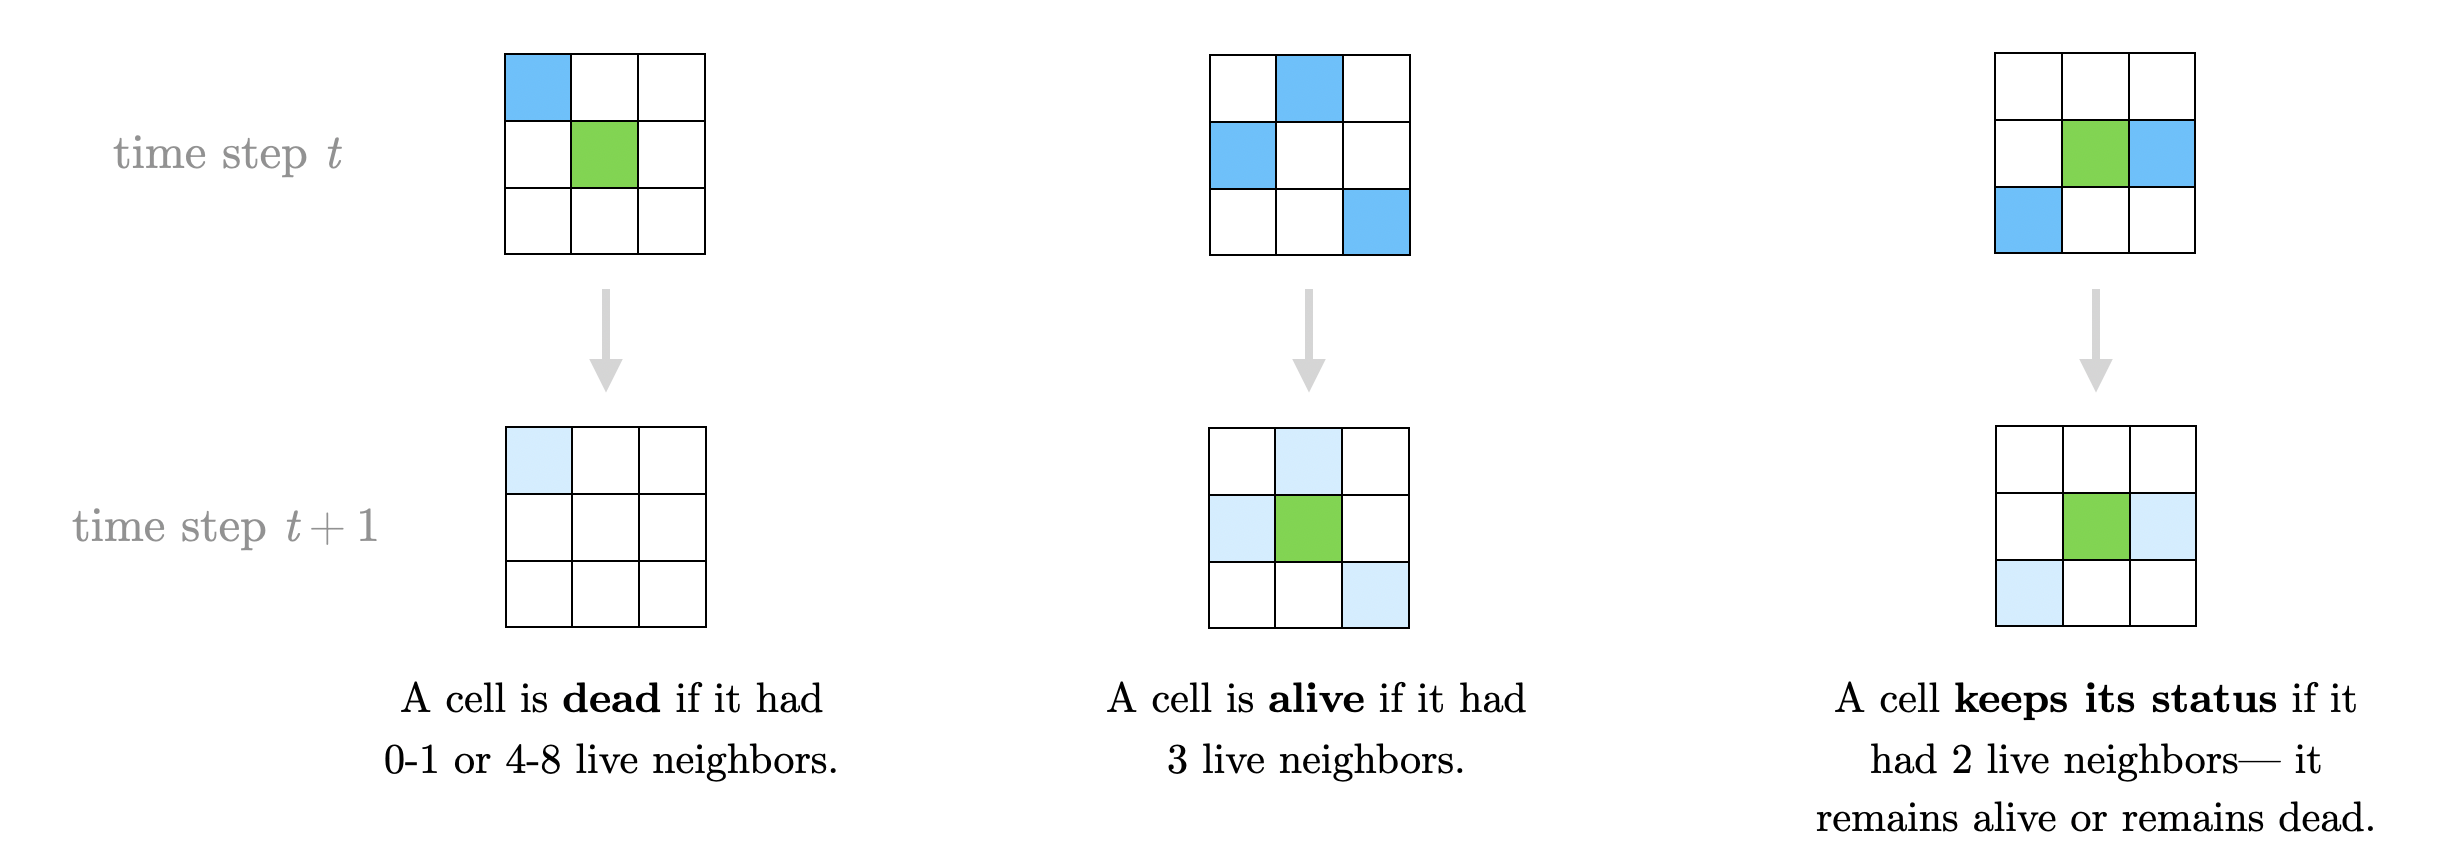
\includegraphics[width=13cm]{gameoflife.png}
\end{center}
Those rules apply to every cell on every time step.

\pagebreak

In such a world, we can make a strong physics-based claim, such as:
\begin{claim}
    Living cell $x$ will remain alive from one time step to the next when 2 or 3
    neighboring cells are alive in the previous time step.
\end{claim}

How could such a claim have any uncertainty?

Unfortunately, it can. Even if we one day discover laws of physics that
explain every experimental result throughout all of human
experience, we're still making two fundamental assumptions:
\begin{itemize}
    \item We're assuming that any laws of physics exist at all.
    \item We're assuming not only that laws of physics exist, but that they
        remain unchanged throughout all of time.
\end{itemize}
As much as we may {\em believe} these assumptions are true, we do not truly {\em
know}, with certainty, that they must be true.

However much we understand the present, we know nothing about
the future with certainty.

The idea of verifiable truth is so general that we could consider using it as
{\em the} definition of truth.
But there are some truths that don't clearly correspond with this definition.
For example, mathematicans don't accept a theorem as true no
matter how many times you test it and find it to be true --- they require
more than repeated experimentation.
And there are other interesting ideas we call true
which don't fit nicely under the umbrella of verifiability.
Consider the claim:
\begin{claim}\label{c2}
    Han shot first.
\end{claim}
This is in reference to Han Solo's encounter with the bounty hunter Greedo in
Mos Eisley, as depicted in the 1977 film {\em Star Wars}.
In the original version of the film, Han Solo clearly shot Greedo before Greedo
had a chance to
fire at Han, but in later, edited, versions of the film, Greedo either shot at
Han first or nearly simultaneously. So the truth of claim \ref{c2} is not
obvious.

I don't think claim \ref{c2} can be verified to the degree we can verify
water boils at 100\degree C.
It's about a fictional event in a widely-known story.
For many narrative-based questions, we could simply ask the author since they
have a kind of authority over what ``really happened'' in the story they
created. But in this case, the story of {\em Star Wars} has effectively
graduated to a level of American mythology, in which case the authorship of a
single living person (George Lucas, in this case) is less meaningful.
The ambiguity of ownership causes some ambiguity of truth;
this shows that our belief in some ideas depends on an agreed-upon author.

Let's call claim \ref{c2} an {\em authored idea} --- it's an idea whose
truth depends on decisions by an author.
This applies to ideas from fictional stories with an agreed-upon
author, but it also applies to things like laws or standards, which are often
decided by groups of specialists. For example, the default text encoding of the
web is to use Unicode code points, which provide a way to encode most of the
world's writing systems. The Unicode Consortium is an organization that's
recognized as deciding all the details of Unicode.
While no person or group can decide the value of $\pi$, the Unicode Consortium
can decide which emoji are included in Unicode, and therefore available on your
phone.

Let's officially define this new kind of truth:
\begin{defn}[Authoritative Truth]
    An authored idea is true when the party recognized as the authority confirms
    the idea.
\end{defn}

We could ask if Harry Potter likes cilantro. This question is not addressed in
any of the writings of author J.K.~Rowling. However, if she were to publicly
declare the answer one way or another, it would be accepted as canonically true.
Just as much as we accept the statement ``Darth Vader is Luke's father,'' we
would also accept ``Harry Potter loathes cilantro.''

Ideas about fictional entities may feel less real,
but there's still a feeling of rightness or wrongness to them.
If a kid asked you where Santa Claus lives, you would tell them he
lives at the North Pole. There is a shared narrative here; if you were to say he
lives at the South Pole, this would feel incorrect.

While fictional stories are not about things that happened in reality, when we
talk about these stories, we're still talking about actual events. The telling
of the story,
the experiencing of the story, and our discussion and thoughts of the
story are all real events.
If the story has enough appeal,
then it becomes something greater than a single telling.
Stories,
to humans, are a part of our experience and our learning in terms of what can
happen, how people behave, and how we learn about life. Our own thoughts and
actions evolve as we experience narratives, whether they are our personal
experiences, those we know of our community, or those stories we hear
indirectly.

For example, we generally do not learn that murder is bad by committing or
witnessing murder. Instead, we learn about it as we grow. In some cases, we may
hear stories of loss, and at some point, vicariously experience some pain of
loss that helps us to appreciate the harm of taking a life.

To me, moral ideas never feel black and white, but so many people consider them
to be such that I'll include this kind of truth:
\begin{defn}[Moral Truth]
    A moral guideline is true when a society following it is better off than a
    society that ignores it.
\end{defn}

There's a lot in that definition. I've chosen to work with a variation of
Immanuel Kant's categorical imperative --- his style of the golden rule. It's
quite a rabbit hole to consider this definition carefully, so for now I'll ask
you to accept that we're not focusing on morality, but rather noticing that if I
say ``murder is wrong,'' this is an idea which we may say is true or false, and
which is more clearly a {\em moral truth} than the other kinds of truth in this
article.

There is yet another kind of truth adjacent to morality. Consider the claim:
\begin{claim}
    Forks go on the left side of your plate.
\end{claim}

There is a sense of agreement about this claim, and yet it is clearly not a
result of a logical argument, nor of a physical experiment. Neither is it
a moral directive since no one seriously suffers
if a fork is placed to the right of a plate.
There are other truths not far from this kind, such as
the convention of wearing certain kinds of outfits to a wedding or a funeral.

It's interesting that these conventions are not understood as a single
{\em correct} way to do things, but rather they represent a
{\em consistency} within a group of people.
In the case of utensil etiquette, the consistency provides an expression of
cultural status and awareness; proper wedding attire conveys respect for the
event and the people getting married.
What makes a convention correct is an understanding of what most people expect.
In other words, the truth of these things is based on noticing what
the majority already treats as the correct decision:
\begin{defn}[Democratic Truth]
    A social convention is true when the vast majority of a society consider it
    to be true.
\end{defn}

It's not always obvious how democratic truths form.
Did a monarch one day
see a fork on the right of her plate, felt funny about it, and decapitate her
table-setting staff members?
Perhaps from that day forth, forks were carefully
placed on the left.

This possible fork-on-the-left origin story is an example of an idea being
decided by a single individual.
In some rare cases, it does seem as if a single point of history determines a
convention.
Consider the sandwich.
The word {\em sandwich}, referring to food, is distinctly traceable to John
Montagu, the $4^\text{th}$ Earl of Sandwich. The story, provided by plausible
historical accounts, is that he liked to eat quickly and cleanly while either
gambling or working (depending on your source), and a bread-enclosed meal did
the trick.

More often, it appears that conventions evolve slowly. Rather than arising from
a single conscious decision, they appear to be an accumulation of natural
smaller steps, with a reason behind each step.
These might not always be {\em good} reasons,
but
when you examine the history of a concept,
you often find more sense
than you might expect. Newts were once ewts; when people saw one they would tell
their friend they saw ``an ewt,'' which was so easy to confuse with ``a newt''
that the word changed. People once considered the Mediterranean Sea to be the
sea in the middle (medi) of the earth (terran).

In the examples above, we're seeing ideas, like words, that live in multitudes
among communities --- such as French words in France, or mathematical lingo
among mathematicians. These ideas shift and adapt as the world changes.
Some ideas receive more attention while others, apparently less useful, dwindle.
This brings us to another perspective on truth that's worth
consideration in its own right:
\begin{defn}[Evolutionary Truth]
    A communal idea is true when the persistence of that idea corresponds
    with the persistence of the community.
\end{defn}

Peculiarly, this definition doesn't directly convince us that an idea
corresponds to reality. This may irk your intuition.
Yet, by this definition, every good idea is evolutionarily true.
For example, if one community believes in germs, and another
doesn't, then over time the germ-believing community is more likely to survive,
and the concept of germs with them.
Ideas are the social genes of the community.
They mutate and change over time, and the theory of natural selection
applies to ideas just as they do to traditional genes in a species.

At the same time that good ideas tend to be evolutionary truths, there's room
for other ideas to tag along for the ride.
While good ideas are evolutionary truths because they promote survival, other
ideas may count as evolutionary truths simply because they are good at
keeping themselves alive, rather than keeping the community alive.
Some beliefs of organized religion seem to fit into this category.
Religion historically helped communities
by encouraging them to work together, to help each other
out, and to remain organized. Those are genuine benefits. Along with those
benefits came ideas that do not correspond with reality, nor do they confer
verifiability or utility in practical decisions. One example is the belief that
Zeus exists as a god, and is the son of the titans Cronus and Rhea.

You might say that these religious beliefs are authoritative truths.
But believers are likely to disagree, saying that the authority of a
religion derives from it being true, and not the other way around.

Just as there is uncertainty in the previous kinds of truth, there is
uncertainty here.
Indeed, there are many incompatible religious beliefs, so they simply
cannot all be correct at the same time.
In other words, it's perfectly possible for an idea to persist in a community
even when that idea doesn't meet our intuition for being true.

\subsection{Which definition is right?}

As we work through these kinds of truth, it's tempting to ask:
\begin{question}\label{q3}
    Is there a single all-encompassing definition for truth?
\end{question}
In other words, is one of our definitions the {\em main} definition, with the
others describing subsets of truths?
Just as we can provide multiple definitions of an English word, I think there
is more than one valid definition of truth.
Even in mathematics, we can sometimes
define a technical concept in different ways, and those
ways end up being equivalent after some analysis.
Accordingly, I'll provide more than one answer to question \ref{q3}.

First I'll argue that:
\begin{answer}{3a.}
    When we seek to describe the truths that groups of people tend to believe,
    we're talking about evolutionary truth.
\end{answer}

This answer is almost tautological in the sense that I'm aligning the context of
the answer with the definition of evolutionary truth.
Still, there's
an interesting thought here: we're taking the vast wealth of work on
biological evolution and seeing that it applies to what we accept as true.
Proponents of this notion include
biologists such as W.D.~Hamilton and
Richard Dawkins, who consider evolution to apply to ideas in
social settings.

Based on this perspective, humans
may deserve less credit than we tend to give ourselves for having many
brilliant ideas. Just as evolution created life, flight, eyeballs and
brains without individual insights, perhaps the simple mechanism of billions of
people guessing and checking many possibilities deserves some
credit for human innovation.

Among our definitions, evolutionary truth stands out because it describes
ideas that are believed, yet it doesn't
care about individuals' justifications for the ideas.
This distinction is a bit like the difference
between language that is correct in theory, such as the grammatically
correct phrase ``that's neat,'' versus
langauge that is used in practice, such as ``it's lit fam,'' having roughly the
same meaning.
When we have an opinion about the correctness of something (such as the
proper linguistic structure of ``that's
neat''), we have a {\em
normative}, or judgment-oriented perspective.
If we are observing
without judgment (noticing that ``it's lit fam'' is used in reality),
our perspective is {\em descriptive}.
Evolutionary truth is our descriptive definition of truth.
It is more about how ideas survive than it is about what an omniscient being
would agree with.
With that in mind, it's tempting to consider which ideas survive even
if they're not correct by any other definition of truth.

Which definition of truth might be a good benchmark to filter out truly
good ideas from ones that are persistent yet unhelpful?
Consider this final definition:
\begin{defn}[Effective Truth]\label{d8}
    A useful idea is true when someone using it tends to achieve their goals by
    doing so.
\end{defn}

For example, suppose you believe that red bowling balls are luckier than any
other color. It just so happens that your red bowling ball fits your hand better
than your other one, which is orange.
In this case, your belief helps you to
achieve higher bowling scores, so it's effectively true.
I've chosen this example to pique your sense of imperfection, but next I'll
argue that all of our ideas are like this; that is, I don't think the
imperfection is in the definition of effective truth,
but is a necessary property of truth itself.

Consider the simple and useful formula:
\begin{claim}[Newton's second law]
    $F = m \cdot a.$
\end{claim}

Unlike your belief that red bowling balls are lucky, this idea probably feels
unsuperstitious and reasonable. Here's the thing: it's not true.
Newton's laws only apply to non-tiny
objects that aren't moving very quickly (a physicist would say Newton's laws
apply when the speed is slow enough to be called non-relativistic).
Even under those conditions,
it turns out Newton's laws are only approximations due
to relativity.

How is Newton's second law really different from the idea that red bowling balls
are
lucky? There is a difference in that, if we were to scientifically explore both,
we'd find one of them is, as an approximation, correct much more often than the
other. Can we say that one is true and the other is false? I don't think so;
both will fail to be perfectly true in many experiments. And both will appear
more true than chance in the contexts above.

What we end up with is a way to evaluate different shades of truthiness.
This perspective of truth relies on the context of goals to make sense.
A ``very true'' useful idea, given
a certain goal, will achieve that goal almost every time. If a goal can
almost never be achieved, then we may still care about ``slightly true'' ideas
--- ones which achieve their goal only a small percentage of the time;
consider a drug that saves 2\% of patients with an otherwise fatal disease.

Similar thinking also works for evolutionary truth in the sense that if an idea
is very persistent, then it better fits the definition of being evolutionarily
true. In both cases --- for both effective truth and for evolutionary truth ---
there are degrees to which an idea is true or false.

Here's the theme of this article:
Truth is not as straightforward as we'd like it to be.
It's worth spelling out clearly how we can measure degrees of truth in terms of
the descriptive/normative viewpoints mentioned earlier:
\begin{itemize}
    \item{} [Descriptive perspective.]
        {\bf Communal ideas are as true as they are
        persistent}.
        That is, an idea believed by a community of people has
        more or less evolutionary truth to it according to how well that
        idea tends to persist, meaning both that people agree with it, and
        that those people continue to survive.
    \item{} [Normative perspective.]
        {\bf Useful ideas are as true as they are effective.}
        That is, an idea being used to achieve a goal in a certain context
        is more or less effectively true according to how often someone can
        better achieve the goal by using the idea.
\end{itemize}

I'll summarize this:
\newcommand{\obstwo}{
    For both
    effective and evolutionary truth,
    ideas are neither completely true nor completely false, but have degrees of
    truth.
}
\begin{obs}\label{o2}
    \obstwo
\end{obs}

The concept of effective truth is not new, although as far as I know the
particular definition I'm providing here has its own nuances.
Various philosophers have previously
explored similar approaches to truth, including Charles Peirce and William
James; their line of thinking is referred to as {\em pragmatism}.

Is effective truth the same as our human intuition for truth?
Something at first feels mismatched, and I'll explain this mismatch as an
objection to effective truth.
We want an idea to be true when it describes how the world is;
it feels like achieving a goal is secondary to being
correct about the world.
Here's an example idea: A cloudless daytime sky is blue.
It seems there's no goal to be achieved by knowing the sky is blue,
so the idea is not effective (it's not goal-based) while
still being true.

Here is a response to that objection:
Although the idea the-sky-is-blue does not itself specify a goal, there
are many goals I can achieve with that idea. For example, I can paint a
landscape picture that includes the sky.
I can look up and determine if it's likely to rain or not.
If I can succeed in achieving my own goals by making use of an
idea, then that idea has been effectively true.
Later, in observation \ref{o4}, I'll argue that we cannot even think of ideas
unless they are somehow associated with some goal.

Another objection to effective truth can be found in thinking that red bowling
balls are lucky.
If I only have a red bowling ball and an orange one,
and there's
something wrong with the orange one, then my belief that red bowling balls are
lucky becomes effective for me.
Yet it feels wrong, because it doesn't feel true
that the color of a bowling ball can directly increase my bowling scores.
In general, perhaps we achieve a goal by doing a good thing for a bad reason.
In that case, the idea could be effective, but doesn't match our intuition about
what a true idea is.

Every time we put an idea to the test, we use it in a way that will either
confirm the idea or refute it. Different tests may reveal different aspects of
the idea. For example, if we try to apply Newtonian mechanics to
near-light-speed space travel, we'll find physical experiments where an
observation directly contradicts Newton's laws --- that is, Newton's laws will
be wrong.
When we find a new context where an idea is wrong, we have to either
label the old idea as false, or to modify the idea to
better understand where it applies.

In the case of red bowling balls, when applied to the single choice of the red
versus the defective orange bowling ball, the idea of red being lucky simply
works. The phrase ``is lucky'' is vague, but in this application, it
means, ``I usually get a higher score when I do this.''
If we tried to apply that same idea to other bowling balls then we would have to
either discard the idea completely or add a restiction to it --- just as
Newtonian mechanics needs to be qualified.
In other words, if you believe
the laws of Newtonian mechanics have some truth, then you must likewise accept
other qualified approximations for reality as true in the same sense.

% Every idea is uncertain and ---
% using our earlier uncertainties about
% math and logic --- we can always doubt the
% correctness of its reasoning. Thus:
% \begin{obs}
%     Every idea is approximate; there is no meaningful distinction between good
%     reasoning or bad reasoning beyond testing the ideas to be compared.
% \end{obs}
% I do not mean to disregard a widely-accepted argument. I do mean to say that if
% we have two ideas which reach the same conclusion, and both lines of argument
% are equally accepted, then there is no way to distinguish which line of
% reasoning is better than the other. 

I think that effective truth corresponds to our day-to-day intuition for truth.
Here's a general argument to support this:
\begin{argt}[That effective truth matches our intuitive idea of truth.]
    \label{a1}
    \normalfont
\begin{itemize}
    \item[]
    \item For every idea, we can only understand its truth by making decisions
        with the idea and seeing if the decisions result in things we expected.
        I call this {\em testing the idea.}
    \item{} [{\bf Case 1}]
        Suppose an idea will pass every test we ever give it. Then
        the idea
        matches our intuition for being true, and simultaneously matches the
        definition of effective truth.
    \item{} [{\bf Case 2}]
        Suppose there is some test which the idea would fail.
        Then the idea fails the definition of
        effective truth, and also fails to be seen as perfectly true by our
        intuition.
    \item{}
        {\em Note:} There is no room for discoverably
        bad reasoning (``red is lucky''):
        If a line of bad reasoning is discoverable,
        then there is a test that can reveal the incorrectness
        (eg, scientifically test all red bowling balls, and we find that red is
        not, in fact, lucky).
        If the idea
        relies upon undiscoverable bad reasoning (``because souls are purple''),
        then the undiscoverable part of the idea is superfluous and has no
        bearing on decisions or outcomes; thus we can ignore it and focus on the
        parts of the idea which allow testability.
\end{itemize}
\end{argt}
Thus, to simplify, there are only two cases, and in both cases our intuition is
found to match effective truth. To unsimplify, we must face the reality that (a)
many useful ideas are known to be simplifications or only partially true; and
(b) that, even if an idea has passed every test so far, we cannot know if it
will continue to pass all future tests.
We'll return to those two caveats below.

I'll summarize the above discussion as:
\begin{answer}{3b.}
    Our practical intuition for truth matches effective truth.
\end{answer}
I've included the word {\em practical} here to separate this kind of intuition
from a more {\em mathematical} intuition that we also have for truth;
I'll briefly revisit this mathematical intuition in section \ref{supertruth}
below.

With answer 3b in mind, the rest of this article focuses on effective truth.

Some philosophers, such as Karl Popper, might prefer the definition given for
verifiable truth over that for effective truth.
I began with verifiable truth because it is a simpler notion that appeals to the
tradition that ideas are either completely true or completely false.
And this dichotomy shows us the distinction between verifiable and effective
truth; effective truth works well with ideas that are only partially true.

How does effective truth relate to the other definitions of truth?
Evolutionary truth is different in that
it allows for kinds of truth which are persistent yet not effective.
The other kinds of truth are special cases of effective truth.
If an
idea is, say, democratically true, then it's effective at achieving a democratic
goal. These special cases of truth have been separated
according to the kinds of goals they achieve. Authoritative truths achieve goals
that standardize ideas using a central deciding authority; democratic truths
achieve goals that align expectations among many people; moral truths achieve
goals that improve society-level quality of life;
and mathematical truths achieve
goals in mathematical settings.

We've ended up focusing on effective truth, noting the special role of
evolutionary truth. I've argued that this matches our key intuition for truth in
that effective ideas give us the expected results when tested. But there are
other intuitions we have for truth. I'll highlight two properties (I'll call
them P1 and P2) that people tend to believe about truth:
\begin{claim}[Spoiler: I will disagree with this.]\label{c7}
    An idea being true is:
\begin{itemize}
    \item{} {\normalfont [{\bf P1.}]}
        {\bf Independent of minds.} That is, whether an idea is true has
        nothing to
        do with anybody asking the question.
    \item{} {\normalfont [{\bf P2.}]}
        {\bf Context-free.} That is, whether an idea is true does not depend
        on
        how we think about or test the idea.
\end{itemize}
\end{claim}
Effective truth seems to be at odds with these properties:
Effective ideas are tied to their believers and their goals in that
an idea's truth depends on believers' actions and interpretations.
The remainder of this
article explores the relationship between ideas and believers.

\section{Inventions}

A simple model of the world breaks all things down into {\em inventions} and
{\em natural objects}.
A natural object is something that existed independently in the
world before it was found, such as Mars or the gravitational constant.
On the other hand, an
invention is something purposefully made, such as
a car or a song.

For the sake of this article, I'm going to slightly expand
the usual meaning of the word {\em invented} so that it applies
to anything at all that has been purposefully created.
For example,
it's not clear if the traditional idea of invention would apply to birds' nests,
but I'm shifting definitions so that they count as invented since
they're
created by birds to serve the purpose of a
home.
I'm using this adjusted meaning because it handles edge cases that would
otherwise be unclear, and because it's interesting to notice
what's purposefully created and what's not.

With these categories defined,
let's take a look at an interesting invention: an object's
center of gravity.
The philosopher Daniel Dennet calls the center of gravity
a {\em useful fiction}
because it's not a physical part of the world, although it is useful.
It lives in an interesting space between being real and imaginary.
A well-defined solid object always has a center of gravity,
and no human decides where it is.
In this way, the center of gravity
is somewhat independent of human minds.
Yet it does not correspond to any particular molecule within that object.
Just as the financial value of a dollar bill only exists as an agreement between
minds, the center of gravity is an idea, and not a physically separate
entity.
In this way, a center of gravity is somewhat dependent
on human minds to exist.
I'm telling you about this dual nature because
other concepts share this duality, and we'll use this lens to explore
the dependence of truth on the minds of believers.

It's strange to call a part of physics, or to call a mathematical idea, a
fiction. 
I'm using the word {\em fiction}, as Dennet did, in a
nonstandard way.
Instead of meaning that the idea is incorrect, I mean that it is created.

Useful fictions are inventions.
The idea of a center of gravity is something created by
people with the purpose of better understanding physics.
There are many other useful fictions in our universe. To help identify them,
notice that:
\begin{itemize}
    \item A useful fiction $x$ is a {\em fiction}
        in the sense that we can completely
        describe the physical state of the world without needing to describe
        object $x$.
    \item A useful fiction $x$ is {\em useful} in the sense that we, humans,
        accomplish some goal with it.
\end{itemize}
The concept of ownership is a useful fiction, as are the notions of
calculus and of beauty.

You might object by nothing that, based on the points above,
many natural-seeming objects could count as useful fictions.
For example, limestone: In theory, we could describe the full state of the world
in terms of basic particles without any need to actually
define what limestone is. Is something as natural-seeming as limestone really
dependent on minds to exist?

I claim that the concept of limestone --- and other similar, natural-seeming
concepts --- are indeed somewhat dependent on minds to exist.
My formal argument is that anything meeting the two bullet points above for a
useful fiction is something that is goal-motivated, and is based on a conscious
decision within a mind to be named and generalized; and most human concepts have
both of those properties.

I can try to establish some intuition that most human concepts are in fact
dependent on minds to exist. To do so, I'll momentarily pretend that our rules
of physics are based on the game of life; this will sidestep the fact that we do
not yet know the rules of physics of our own world.

In the game of life, the word {\em glider} means a particular 
configuration of cells that moves diagonally across the board, assuming it does
not encounter another object.
% 
% \pagebreak
% 
% \noindent
Here are all the shapes of a glider:
\begin{center}
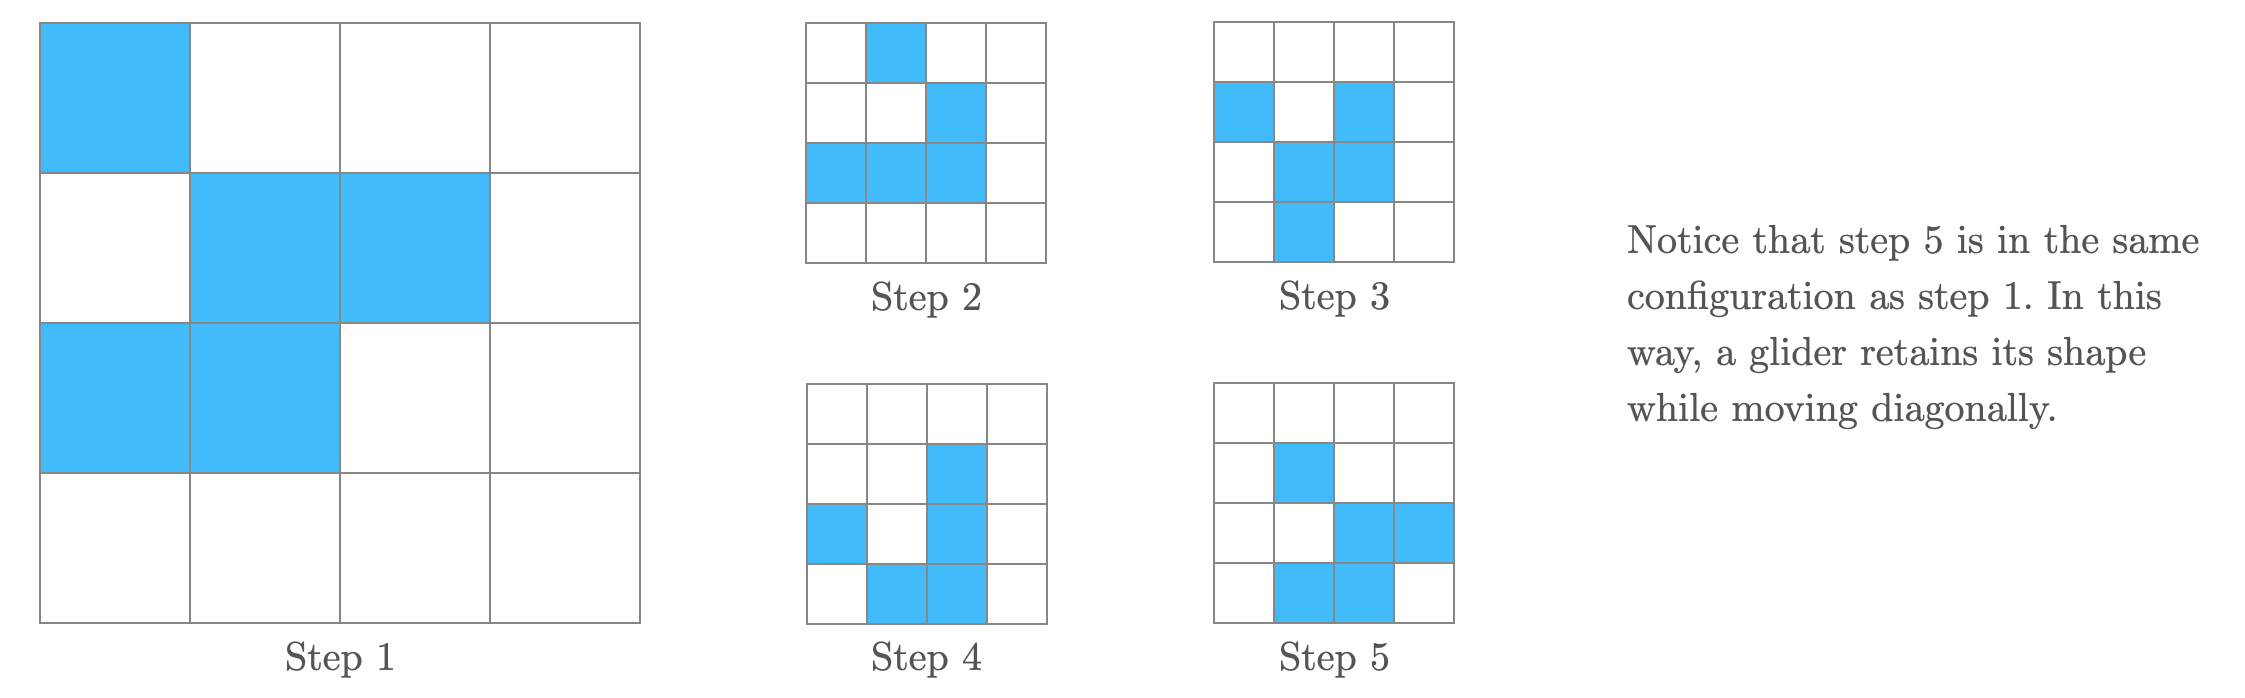
\includegraphics[width=14cm]{glider2.png}
\end{center}
The universe may contain nothing but gliders, yet we still have no need
for the concept of a glider to describe everything in it; we could simply
describe grid cells as being alive or dead.
The glider concept is useful, created, and dependent upon minds for it to
exist. Despite being analogous to a simple molecule, they are still a useful
fiction.

Now let's return to the physics of our own world. Consider the concept of water.
Water seems quite natural;
it would be strange to say it's an invention.
Now consider a hypothetical {\em molecule X} which was painstakingly synthesized
in a pharmaceutical research lab to treat a disease.
Molecule X does not occur naturally on Earth,
and in fact is quite difficult to create. It seems more natural to say that
molecule X was invented.
Why do we freely call molecule X an invention, while we want to say
water is natural?
It seems the difference to us is in the pre-existence of water, and
in the purpose of molecule X.

Now consider a remote planet where molecule X is abundant, but water is
nonexistent. Inhabitants of this planet could reach the opposite conclusion if
they created water themselves. So it seems that our intuition for what is
natural and what is invented depends on our personal experience, and is
not objectively based on the state of the universe alone.

Our judgment of some concepts being natural is itself something
we find useful, and something we have added to the world; it is a useful
fiction.

Here's why I'm discussing all of this:
\newcommand{\obsthree}{
    Truth is a useful fiction. It is an invention, and not a natural part of the
    world.
}
\begin{obs}\label{o3}
    \obsthree
\end{obs}

This observation disagrees with the common intuition from claim \ref{c7} that
truth is independent of minds (P1). How can I justify observation \ref{o3}?

One simple justification is to note that truth meets the two bullet points
above: Truth is not something we need to describe the world, and it's useful.

I'm going to provide more than one argument to support observation \ref{o3}
because it can feel quite unintuitive.
For example, I think it's easier to see that the concept
of falseness is invented, and we can make use of that:
\begin{argt}[That truth is an invention.]\label{a2}
    \normalfont
    \begin{itemize}
        \item[]
        \item
            The idea that ``$x$ is true'' only makes sense as a denial of the
            opposite idea that ``$x$ is false.'' If there were no concept of a
            false idea, then the concept of a true idea would be meaningless.
        \item
            The idea of falseness is clearly invented. We can describe
            the world without having to include the idea of falseness.
            There is a purpose to the idea of falseness, which is to understand
            mistakes or deception.
        \item
            Combining the above two points:
            Since the idea of truth is essentially paired to the idea of
            falseness,
            it must be the case that both ideas are invented.
    \end{itemize}
\end{argt}

A natural counter-argument is that perhaps falseness is invented while truth is
not.
I will expand on this point below in \S\ref{s_mental_words},
arguing that pairs of concepts which are alternatives to
each other can only exist together,
rather than individually.

\section{What Ideas Are}

In order to better understand the relationships between alternative
notions (up vs down, red vs orange, true vs false), it's
helpful to begin with the question:
\begin{question}
    What kind of thing can be true or false?
    In other words, what is an idea?
\end{question}

So far I've been blithely using the words {\em idea} and {\em claim} to talk
about things that might be true.
As a reminder, the word {\em idea} in this article is adjusted to focus on
clear and meaningful expressions that can be true or false.
So when I say {\em idea}, I'm excluding
things like ``the idea of the color green'' because that isn't something that
could be true or false.

Some philosophers go into a tizzy when you ask
what kind of thing can be true or false (question 4).
You might say a grammatically correct {\em sentence} can be true or false,
but then you must deal with any random yet grammatically correct string
of words
like ``a yellow sadness confused the used
passenger;'' or logical ambushes like ``this sentence is false.''
There's a serpentine rabbit hole here that I don't want to get stuck in.

% OLDTODO vvvv I promise two connections. Ensure this promise is well kept. vv
%   Yes, I do. First connection is made 4.1; second is made in 4.2.
Instead of trying to find a perfect answer, I'm going to speak at a high level
and suggest two connections that help us better understand the word {\em idea}
as it's used in this article.
I'm not going to define exactly what an ``idea'' is.
I'm going to keep the word {\em idea} as a placeholder for our
intuitive understanding of what can be true or false, and I'll lay out some key
properties of this intuitive notion.
% TODO XXX ^^^ Do I make use of this last sentence?

\subsection{Questions and Answers}

The first connection I want to make is between ideas and answers to questions.

If an idea tells us some information, then it must distinguish between different
possibilities. If I say ``I'm having a nice day,'' then I'm distinguishing this
from the possiblities of having an astounding day or a dog-tired day.
If there were no other possibilities,
then there is no information conveyed. If I said
``red is red'' without more context,
it's confusing because it's not clear what
alternative I'm excluding.

There's a nice mathematical analogy here. It's almost as if there were a short
conversation like this:
\begin{itemize}
    \item{} [Mathematician A] I know the value of $x$ is in the set of
        possibilities $X$, but exactly which possible value is $x$?\\
        (The math notation here is to say that $x\in X;$ what is $X$?)
    \item{} [Mathematician B] Oh, it turns out that $x=4$.
\end{itemize}
There is a question (what is $x$?) with a set ($X$) of possible answers. The
information content --- the idea being expressed ---
is an answer to this question ($x=4$). If you say ``My name is Inigo,''
then you are answering the implicit question ``What is your name?'' whose set of
possibilities is the set of all names.

This mathematical analogy is not perfect.
We often speak without thinking about the
alternatives we're excluding.
The question we're answering
is typically implied, and may not be clear, even to
the speaker.
I claim that if you {\em did} think about any statement
you
make, then
you'll typically find specific alternatives you've excluded.
Another imperfection with the analogy is that some sets of possibilities are not
clearly defined.
If I say ``this wine tastes of
elderberries and the phlegm of an incontinent camel,'' then we must admit there
seems to be a fuzziness to the set of things a wine can apparently taste like;
you'd be hard-pressed to enumerate this set exactly.

Nonetheless, the analogy helps us to build our intuition.
An idea has meaning only because it expresses one way things
{\em are} from amongst a
(non-mathematical) set of possible ways things {\em could be}.
Similarly, a question is an expression of a set of possible ways things could
be, along with a desire to learn which item in that set is correct.
I'll summarize this
connection as:
\begin{answer}{4}
    An idea is an answer to a question.
\end{answer}

This is similar to a definition, but really I'm just breaking down
one intuitive notion (ideas) into two other not-carefully-defined notions
(answers and questions). I still find this connection useful, as we'll see
below.

\subsection{Goals}

The second connection I'd like to make is inspired by asking:
\begin{question}
    Why do we ask questions?
\end{question}

Perhaps every thought we think, including every question we ask,
is motivated by a goal.
But there's an objection: It seems that some thoughts
we have are not goal-motivated.
Consider raw perceptions that enter your mind simply because
you experienced something --- for example, you notice a car driving by,
or perhaps you hear a friend ask a question. You may understand
your friend's question without being directly motivated to ask it yourself.

With this objection in mind, I'll separate our thoughts into
{\em conscious} thoughts that we deliberately choose to have,
and {\em external} thoughts or perceptions which we do not choose.
I'll make the claim that every {\em conscious} thought you have
is motivated by some goal you have.

Are there any remaining objections to this claim?
If you try hard, you might come up with interesting 
thoughts that seem to be conscious yet may not have
clear goals. As examples, consider a child at play, or
someone distracted by a squirrel running across their path.
In the case of play, I think that having fun is itself a goal.
Play is an action some animals engage in.
It may be helpful in learning about social interactions and
other life skills.
In terms of being distracted by a squirrel,
I would say the initial moment of distraction is an
external, unbidden thought --- you see a squirrel. However,
if you have any follow-up thoughts about the squirrel, those
are conscious thoughts. They may be motivated by
curiosity, which I see as a basic drive alongside
our need for food or sleep.
Sating your curiosity is a goal.

For any conscious thought I've considered, I've
found a goal behind it.

Based on this, we can have conscious thoughts that are ideas, and others that
are questions. The perspective of this article is that an idea is an answer to a
question, so in either case there is a question present. And a question is a set
of possibilities along with a desire to know which of these possibilities will
help us move toward our goal.

\pagebreak

Let's summarize this as:
\begin{answer}{5}
    Every question we consciously consider is motivated by a goal.
\end{answer}
This includes both questions we ask directly as well as
implicit questions that give meaning to a conscious idea, as per
answer 4.

\subsection{Impossible Ideas}

What I've argued is that every idea is an answer to a question, and that every
conscious question is motivated by a goal. Putting these two together,
every
conscious idea is connected to a goal.

This is a strong claim. One key implication is that we cannot consciously
think of ideas that aren't motivated by a goal.

Note that it's possible for an idea to be associated with different goals.
Perhaps the goal which first led us to an idea is
different from a goal we later associate with it. For example, we may first
think of a water heater as a way to make tea, and later learn how to make
instant ramen with that same water heater.
So my claim is not ``every idea has one goal which motivates it,'' but rather
``every conscious idea must have at least one goal to motivate it.''

It's intriguing that there are ideas we cannot consciously think of ---
those for
which we have no goals. They seem hard to believe in, so it would be
interesting if we could find an example to bolster our intuition.
Consider learning to speak Mandarin when you only speak English.
This is difficult because Mandarin uses {\em tones} --- patterns in the pitch of
your voice --- as a key part of a word's pronunciation.
Two words in Mandarain can have
the same consonant-and-vowel sequence, yet can be
pronounced differently based entirely on their tones.
English-only speakers typically have no concept of a word's tone.
They've learned to understand the consonant-and-vowel sounds in English, and to
ignore other points of data from word sounds. If we imagine a world without
tone-based language, then we can imagine that people would never think of
tones at all. Tones would be an impossible concept --- a concept we were
incapable of consciously conceiving.

This isn't a perfect example of an idea we can't think of --- because we {\em
can} think of it; it's just an unknown concept for some people.
It's not my fault I
gave a partial example.
It's literally impossible for me to express an idea that
cannot be thought of.
But such ideas must exist because we'll never
have experienced all possible goals.
For every goal we never have,
there is the question of how to achieve that goal, and an answer to this
question. We will never think of any of these ideas.

If it helps your intuition, consider an alien race that sees colors we cannot;
their eyes see different wavelengths than human eyes.
They will have many words for ``colors''
that we would not recognize as colors. These colors are another kind of concept
we almost cannot think of.
Again, technically, this example is
partial (hence the word {\em almost})
because scientists can understand what I mean --- and, again, any
example I actually give must necessarily be partial. But if you can stretch your
imagination a bit in thinking of these aliens as having entirely new dimensions
of perception, and we never meet these aliens or encounter this dimension of
perception, then you can begin to envision ideas that we're currently
unable to experience.

\subsection{Concepts}\label{s_mental_words}

We have the rough workings of a model of human thought.
I'll add one more
ingredient to this model.
Earlier, I said that this article adjusts the meaning of the word
{\em idea} to exclude, say, the color green since a color
can't be true or false.
In this section I'll formally introduce the word {\em concept} to talk about
things like colors;
concepts are
the things ideas are made of.
Examples of concepts include
colors and water heaters and letters of the alphabet.
Intuitively, if
ideas are mental sentences, then
concepts are mental words.
As with the term {\em idea}, I won't try to define concepts,
but I will analyze our intuition around them.

To ensure the notion of a concept is clear, let's consider another example.
Suppose one day you're stung
by a distinctive-looking wasp.
A year later, you see a similar wasp, and you
steer clear of it, remembering the sting.
It's not that you have an actual word you can say out loud to name this wasp,
but rather that you have a connection in your brain that can recognize it and
understand that it can sting you.
Contrast this level of awareness to a bug you may peripherally perceive, but
never care about; if you saw such an innocuous bug later, you would have no
associations at all with it.

It's possible that concepts originate in a brain process preceding conscious
thought.
I'm not going to suggest a specific origin story for concepts
because we don't need to understand where concepts come from in
order to analyze them.
I've defined a conscious ideas to be goal-driven, deliberate actions.
I suspect that
the first time we deliberately use a concept, it will be a
part of a conscious idea.
If this is the case, then
as soon as we consciously consider a concept, it's attached
to a goal, and this attachment is unavoidable.

% TODO Consider trying to include the image below within the observation here.

I'll summarize this idea along with the previous section as:
\newcommand{\obsfour}{
    Every conscious thought we have is goal-based.

    \medskip

    It's impossible to think of a goal-free concept or idea.
}
\begin{obs}\label{o4}
    \obsfour
\end{obs}

Here's a diagram summarizing the mental model of ideas used in this
article:

\begin{center}
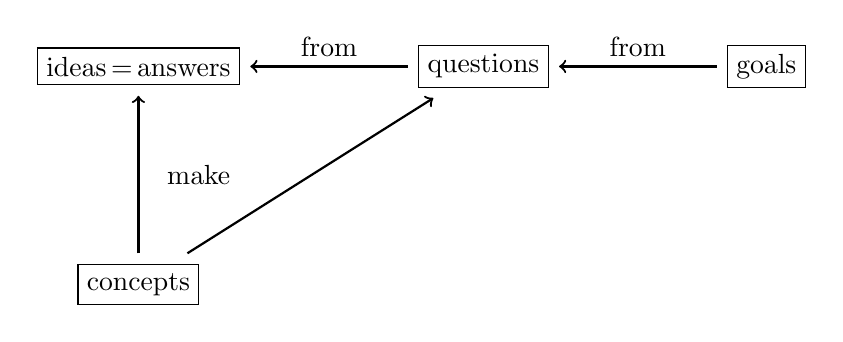
\begin{tikzpicture}[node distance = 2cm, thick]%
    \node (1) {\fbox{ideas\,=\,answers}};
    \node (2) [right=of 1] {\fbox{questions}};
    \node (3) [right=of 2] {\fbox{goals}};
    \node (4) [below=of 1] {\fbox{concepts}};
    \draw[<-] (1) -- node [midway,above] {from} (2);
    \draw[<-] (2) -- node [midway,above] {from} (3);
    \draw[->] (4) -- node [right] {\ \ make} (1);
    \draw[->] (4) -- node {} (2);
\end{tikzpicture}%
\end{center}

In this diagram, I've included the notion that concepts are parts of both
questions and ideas.
This makes sense because a question is the same thing as an idea
with a blank space in it: {\em What is your name?} is the same as
{\em Your name is which $x\in X$?} where $X$ is the set of possible names.

A concept can only add information to an idea if it distinguishes the idea
from alternatives.
There must be possible variations of the idea that are excluded.
This set of variations exists even if it's not clearly defined
If I asked why the chicken crossed the Mobius strip\footnote{Answer: To
get to the same side.\par Note that the corresponding idea, {\em The chicken
crossed the Mobius strip to get to the same side,} seems to pertain to a new
kind of truth not discussed in this article ---
a kind of ``truth'' based on comedic
value, albeit rather hypothetical value in this case.}
the set of possible answers allows for creativity, and is not something we could
easily enumerate.

Some pairs of concepts, like {\em light} and {\em dark}, are essentially
always alternatives to each other.
{\em Heat} has meaning only in opposition to {\em cold.}.
The answer to some questions is expected to be {\em true} or {\em false},
such as when you ask ``Is idea $x$ correct?''
In this way, {\em true} cannot exist alone; it is one concept
together with {\em false}.
This interdependence bolsters argument \ref{a2} above that truth is
an invention.

\scenebreak

Some questions seem less useful than others because we can easily guess their
answers.
For example,
imagine asking a random person if they're
less than 110 years old.
We have concepts for certain age groups such as kids,
toddlers, and teens.
But we don't have a name for people under 110;
that mental notion isn't as useful.
Concepts are useful when they center on
areas of uncertainty, away from predictability.
In other words, there appears to be a correlation between
what we don't know (adjacent to useful questions) and the concepts
related to those questions.
This relationship between truth and ignorance is worth further exploration.

%
% NOTE
%
% The one-word proof that truth is not the foundation of human knowledge:
% hello
%
% Probably rephrase this particular claim to match the proof, but what I mean is
% that we understand actions as more fundamental than truth-bearers.
%
% Slight elaboration: Not everything we do is an idea. Anything we do with an
% idea is an action, but not all actions are things we do with ideas. Actions
% precede ideas in a hierarchy of the human experience.
%


\section{Ignorance and Omniscience}

Ideas depend on questions,
and questions assume ignorance,
even if imagined.
This dependence of ideas upon ignorance
may seem counterintuitive, so
let's try to understand how necessary ignorance
is for ideas to make sense.

\subsection{Ignorance}

I'll use three example questions
to help build up an intuition about the role of
ignorance in ideas and truth.
To state these questions, I'll define
{\em pleven} numbers:
\begin{itemize}
    \item An {\em even} number is any integer that is a multiple of 2;
    \item an {\em odd} number is one more than an even number; and
    \item a {\em pleven} number is any integer which is neither even nor odd.
\end{itemize}
Spoiler
alert: there are no pleven numbers.
But you might be able to imagine they exist, just as you might imagine there can
be a triangle with three 75\degree\ angles before you learn that all triangles
must have angles which sum to 180\degree.
This strange thought experiment is purposefully awkward, and we'll
explore the awkwardness behind it.

Here are the three questions:
\begin{enumerate}
    \item[{\bf Q1.}] How long will my commute be this morning?
    \item[{\bf Q2.}] What's the first positive pleven number?
    \item[{\bf Q3.}] What would the color blue be if it weren't blue?
\end{enumerate}
Question {\bf Q1} seems practical enough. At first glance, there do not appear
to be any strange assumptions behind this question.
Question {\bf Q2}, on the other hand, feels weird because we're asking about
something that doesn't exist. How can we answer a question of detail about a
nonexistant thing? Question {\bf Q3} seems to go one step further in this
direction,
being nonsensical unless we decide to think poetically or
playfully, giving up on taking ourselves literally.

Now, for a moment, imagine that you have complete and immediate awareness of all
future commute times. Suddenly question {\bf Q1} seems silly, a bit like
``How many mintues are in 30 minutes?''
because the answer is obvious to you.
Depending on how profoundly
familiar you feel with commute times, question {\bf Q1} may even feel to you
like ``Is blue blue?'' which is so obvious as to be confusing. If you force
yourself to take seriously the question ``Is blue blue?'' then you're in the
zome of question {\bf Q3}.

Returning to a human who doesn't know all commute times,
question {\bf Q1} is
reasonable because we can imagine worlds with different commute
times. This kind of imagination is akin to ignorance --- to not knowing the
answer.
The other questions are strange because we're deeply familiar with the state of
the world that gives the answers. We can't easily imagine pleven numbers
existing, or blue not being blue.
I included question {\bf Q2} to show how a question's intelligibility
depends on the mind
considering the question. A kid just learning about even and odd numbers will
take this question seriously --- it makes sense to them. But it stops making
sense once you realize there are no pleven numbers.

% TODO Review to see if I consistently use a period at the end of
%      the heading fragments for argument blocks. Be consistent.
I'll summarize this line of thinking as:
\begin{argt}[That ideas only make sense in the presense of ignorance.]
    \label{a3}
    \normalfont
    \begin{itemize}
        \item[]
        \item Every idea is an answer to a question.
        \item A question only makes sense if we can imagine different
            answers are possible.
        \item When we're deeply familiar with information that
            provides the answer, the question no longer makes sense.
        \item Therefore, questions --- and their corresponding ideas --- only
            make sense when they're about things we can imagine not knowing.
    \end{itemize}
\end{argt}
This is a refutation of true ideas being independent of minds (from
claim \ref{c7}). Ideas themselves need the ignorance of minds before they can be
conceived as meaningful.

% TODO XXX Eventually provide an Observation environment that fully refutes
% claim 7, or whatever refutation thereof I feel comfortable with.
% I like the principle that the key claims of this article are highlighted
% nicely in observation brackets.



% One resulting argument is something like if we knew the answer, we would not
% understand the question. In this way truth is dependent on minds.
%
% I think to refute the other side of claim 7 is another place. Some things,
% like 1+1=2, just feel true no matter what. BUT the more interesting truths to
% us are those that we feel more unsure of. We have a hypothetical model of the
% world in our mind, and we don't know for sure how everything works. We imagine
% that if we take action A, we get result A; B->B, etc.
% Any generalization of an idea, any concept of a pattern,
% is based on the imagination that reality could
% have been any other way. If we live in Conway's game of life, then we think
% understanding the rules is meaningful, but in some sense it's no better to
% know the rules than to know all of history. 
%
% I think what I'm leaning toward is something like: We will almost always end
% up with "bad reasoning" like "red bowling balls are lucky." But it's not 100%
% bad reasoning. It's more like, the reasoning will typically be bad when we are
% in areas of high uncertainty. The least assumptive idea is something like if I
% do action A in exact context C then I get result B.
% But for this to be re-usable we necessarily need context C to be changing --
% at very least, eg, we want the timestamp in C to be different. I'd also argue
% that we don't know how to preserve other aspects of the context. An analogy
% could be not knowing which basis is meant in a vector space when we change
% "only the y coordinate;" we could think in terms of an ideal gas law, or in
% terms of asking patients to eat fewer bananas.
%
% I'd say that in situations where we are learning the most, that we also have
% the least understanding of the other variables to control for. How can I argue
% for exactly this? If something is reliable, then we understand it well, and we
% don't think about it much. I don't worry much about addition of small numbers,
% or about quantum physics when playing pool. But there are many problems where
% I have many unknowns. When I raise my kids, how often should I let them take
% small risks? How can I help them see that sugar consumption is not healthy
% despite their lack of maturity and the deliciousness of sugar? These are
% realistic and challenging goals, and it's tricky to even know all the
% variables. Another example might be choosing a nutrition plan, or designing a
% physics experiment.
% 
% Iteration:
% Suppose determinism. If not, then either we have no influence over the outcome
% - nothing to learn - or it's a probability distribution, in which case we can
%   consider the probability of a good outcome as the outcome itself, and then
%   we're back to determinism.
% If there were truly only one variable in a repeatable setup, then it's
% actually not very hard to learn. Why not? Technically, it could be quite
% complex, such as effectively having many different variables encoded into a
% single variable. But then this feels like it's not truly one variable. So for
% the term 'single-variable' to be useful, I think what we mean is an outcome
% that is something like "mostly absolutely continuous" in terms of the input.
% To be a mathematician, I'd say piecewise absolutely continuous where the
% number of pieces is not too large. Then we can do a few experiments and
% typically we will understand the relationship completely. The more variables
% there are, the harder the problem is. The questions we care most about are the
% ones with interesting goals but that are challenging. And in these cases, the
% context is critical. Attached to this argument is the idea that if we
% literally controlled for all variables except for one, then we would be
% limiting ourself to a single experiment (time is a variable, and even if not,
% we'd require a reset of the entire world).
%

\subsection{Omniscience}

% TODO Work on this intro and ensure segue from above.

I'll describe a thought experiment that further explores
how ideas relate to the limits of our awareness.
The general idea is to imagine that you know everything.
Pretend
you're so familiar with the state of the world that questions tend to
feel like ``Is blue blue?'' The answers seem self-evident.
This is
different from knowing the axioms of math and being asked if a certain theorem
is true --- in that case you would have enough information to derive the answer,
but you'd have to think about it first.
I'm aiming for knowledge without the need for additional thought to answer
questions.

To solidify the thought experiment, pretend the world is a single instance of
Conway's game of life. Any single time step is represented by a 2D grid of cells
that are on or off.
Visualize a 3D version of this where each slice is a single time step. In this
way, all of timespace is laid out before you as a single static object. Time is
no longer a mystery, but rather a dimension just like space.

\begin{center}
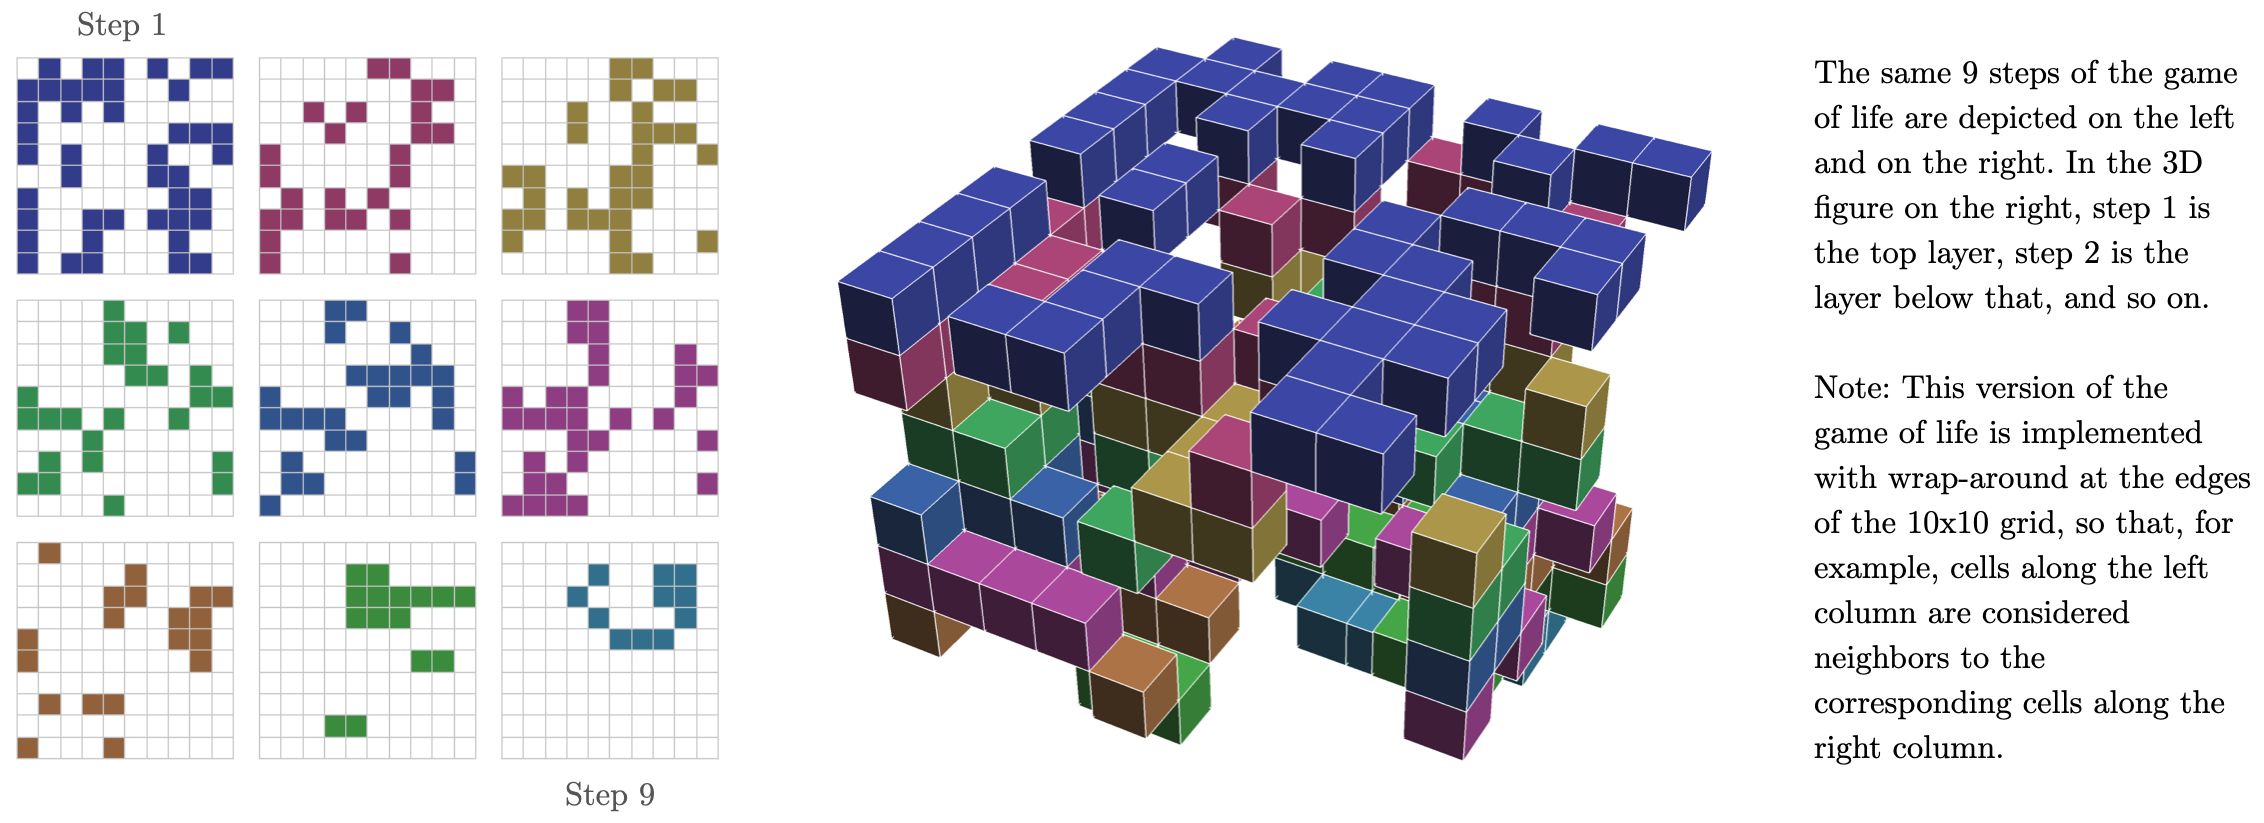
\includegraphics[width=\textwidth]{gameoflife_3d.png}
\end{center}



Hence you ``know everything'' in the sense that you know the full physical state
of the world. Perhaps you don't know all possible mathematical truths, or all
other possible worlds. So this is a certain kind of omniscience. Let's call it
{\em physical omniscience}.

Now someone asks you a {\em physical question}, by which I mean
a question about the physical state of the world.
They point out a glider at a certain time step and
ask how long this glider will live. You, being physically omniscient,
respond:
``What's a glider?'' There's no reason for you to know or care about what a
glider is because you can see all of history without knowing that concept.
Once you
learn what a glider is, then you can easily answer the question. But such a
question feels arbitrary to you, in that a questioner has defined some
random-seeming concept and asked a question about this concept in a situation
where
the answer is inevitable. It may feel as if someone defined even and odd
numbers, and started to go through all the primes checking to see if each one
were odd and even. It's a silly task when you know that 2 is the only
even prime. But it doesn't feel as useless before you know that.

Let's summarize this idea as:
\begin{equation}\label{eq1}
    \text{\em Physical questions seem nonsensically obvious to the physically
    omniscient.}
\end{equation}

Now let's imagine that you are both physically omniscient, and that you identify
with one particular agent in the world.
When you see this agent in the world you
think ``Hey, that's me!'' What kind of goals might you have for this agent? I
don't think you can have {\em any} goals, because you see before you the
full life of your agent just as you see the indelible ink on a page. To imagine
a different path is to reread The Lord of the Rings and hope that Gollum
becomes an insurance claims adjuster by the end. If you're creative, you may
choose to ignore what you already know, but your rational mind understands the
futility:

\begin{equation}\label{eq2}
    \text{\em The physically omniscient are not personally motivated by
    physical goals.}
\end{equation}
 
I say {\em physical goals} to tease out other goals that we can imagine, such as
proving a mathematical theorem. We may also imagine that you, the omniscient
party, exist in some outer world, outside the confines of the world you have
omniscience about (think The Matrix).
You might have agency in this outside world, but that agency doesn't matter here
since the point of this thought
experiment is to look at how knowledge of {\em our} world affects ideas {\em
about our world}, not about other worlds.
That is, {\em physical goals} in (\ref{eq2})
are restricted to actions and results observable
within your inner world, the one that you know all about.

When you know the full physical state of the world, it's
like listing all possible worlds $\{x_1, x_2, \ldots\}$ in a giant list, and
then learning which possible world is the real one. When you're omniscient, you
know there's a certain number $k$ that indicates the real world $x_k$.
If the world used the game of life as the rules of physics, then perhaps the
number $k$ would indicate the starting conditions of the world; everything else
follows. No matter what the rules of physics are, we can suppose there is some
way to encode the state of the universe across all time, and the number
$k$ can be this encoding.

Building on the idea of encoding the world in a single number,
I'm going to pose a strange-seeming mathematical question whose purpose is
(a) to show that some math questions make us wonder what the
point of the question is, and (b) to point us toward understanding the role of
curiosity and abstraction in our thoughts.

Given any positive integer, I can write that number in base 2, in base 3,
etc.\footnote{We normally write a number, like 7, in base 10 because we have 10
fingers, and thus 10 digits (0-9). If humans had only 5 fingers in total, then
we'd have
digits 0-4 and we'd count like this: 0, 1, 2, 3, 4, 10 (this means 5 to us), 11
(meaning 6), 12 (meaning 7), etc. Base $b$ notation is how we'd write numbers if
we had $b$ fingers instead of 10. If this notion is entirely new to you, it's
too much to learn in a footnote, and I recommend googling ``introduction to
number bases'' to learn more.}
I'll create a table by writing a number's base 2 (binary)
form in the top row,
and then below that its base 3 form, then its base 4 form, and so on, keeping
them all right-aligned. Here's a table for the number 534:

\begin{center}
\begin{tabular}{cccccccccc|c}
  &   &   &   &   &   &   &   &   &   &\em base \\
1 & 0 & 0 & 0 & 0 & 1 & 0 & 1 & 1 & 0 & \it 2 \\
  &   &   &   & 2 & 0 & 1 & 2 & 1 & 0 & \it 3 \\
  &   &   &   &   & 2 & 0 & 1 & 1 & 2 & \it 4 \\
  &   &   &   &   &   & 4 & 1 & 1 & 4 & \it 5 \\
  &   &   &   &   &   & 2 & 2 & 5 & 0 & \it 6 \\
  &   &   &   &   &   & 1 & 3 & 6 & 2 & \it 7 \\
  &   &   &   &   &   & 1 & 0 & 2 & 6 & \it 8 \\
  &   &   &   &   &   &   & 6 & 5 & 3 & \it 9 \\
  &   &   &   &   &   &   & 5 & 3 & 4 & \it 10 \\
\end{tabular}
\end{center}

I can make such a table for any number.
I can further imagine that each number in the table is the value of a cell,
analgous to the cells in the game of life being on or off.
I can think of the
top row as the first time step, and as each subsequent row as the next time
step.
(Notice how the number 534 effectively encodes and captures this entire
world; this is ``world 534'' in some sense.)
Now I can ask a question like:
{\em How long does the 1 in the second-from-right column survive?}
That is, if I repeat the top row like this:
\begin{center}
    1 0 0 0 0 1 0 1 \fbox{\bf 1} 0
\end{center}
then how long does the framed cell
remain as a 1 in the rows below?
The answer, for 534, is that this value survives for the first 4
time steps, corresponding to bases 2--5.

As promised, I hope that you have two reactions to this question, corresponding
to earlier goals (a) and (b) of this thought experiment:
\begin{enumerate}
    \item I hope you find this question to be pointless. How is it useful?
        Why would we ever ask this question?
    \item I hope you wonder:
        Out of curiosity, are there any fun mathematical patterns to questions
        like this?
\end{enumerate}

\pagebreak

Now consider the similarities between these questions:
\begin{itemize}
    \item{} [In reality] How long will this person live?
    \item{} [In Conway's game of life] How long will this glider live?
    \item{} [In a number base table, as above] How long will this value survive?
\end{itemize}
These questions all have the same shape: They each specify an
object in the world, and ask how long it will be around.
We probably have different emotional reactions to the questions, but they feel
like the same kind of question to the physically omniscient.

I've
purposefully chosen a well-motivated question (How long will I
live?) to illustrate that even a strong sense of motivation can evaporate
in the presence of physical omniscience.
The number base question (How long will the 1 survive?) is
pointless because you have no control over it or interest in it.
Similarly, your sense of personal agency
and your physical goals both dissipate when your experience of the world is
based
on universal physical knowledge. Questions about survival collapse into the
realm of passive observations, akin to remembering a past event that has no
bearing on the future.

\begin{equation}\label{eq3}
    \text{\em Physical concepts seem pointless to the physically omniscient.}
\end{equation}

The idea of {\em curiosity} throws a wrench into this simple perspective because
virtually any question that can be asked can be motivated, in theory, by
curiosity. If you're physically omniscient and curious, you might find all
questions to be motivated.\footnote{I suspect curiosity has an evolutionary
origin that connects it with survival. For example, perhaps a curious pre-human
primate would discover the utility of controlled fire, whereas a less curious
species would not. This article won't try to analyze curiosity, but I think it's
something we could analyze and put boundaries around. We humans find some things
more interesting than others, and there are probably ways to understand this.}

One thing we can do to fit curiosity into this model is to consider two kinds
world: the physical world, and the world of abstract thought.
A historic fact is an idea about the physical world, while a mathematical
theorem is an idea about the abstract world.
Many ideas blend these two worlds together, such as asking if a particular
theory of physics is true. In that case, we imagine a possible world based on a
physical model; this model lives in the abstract world. And we ask if this model
is a good approximation for reality; we can do a physical experiment to check.

Whenever curiosity is the motivation for a physically omniscient person, there
must be an abstract mental word involved. If there were not, then there is
nothing unknown that makes sense as a question --- we get back to
``is blue blue?'' which invokes no curiosity. And once we're looking at abstract
notions, then we're outside the realm of physical knowledge.
If we wanted to, we could change the thought experiment to imagine a person who
knows all physical states of the world {\em and} all abstract ideas as well. I
think that such a person would then be incapable of curiosity, as no question
could possibly motivated. Indeed, all questions would seem nonsensically obvious
to such a being. Sounds like a disappointing existence.

% TODO See if I can somewhat clean up the statement of this observation.
%      A good result would be if it reads more intuitively and impactfully
%      even to someone with a bit less context. In other words, keep it true to
%      my intention, yet also get across the depth of the idea to people who are
%      just skimming the observations for review after a long time or a first
%      time.

I'll summarize the ideas of this section and the previous one as:
\newcommand{\obsfive}{
    We have no motivation for ideas or mental words without ignorance about
    them.
}
\begin{obs}\label{o5}
    \obsfive
\end{obs}

The omniscient thought experiment also leads as to another argument that truth
is an idea we created for a purpose:

\begin{argt}[That truth is an invention]
    \label{a4}
    \normalfont
    \begin{itemize}
        \item[]
        \item If we can fully describe the phyiscal world without
            mental word $x$,
            then $x$ must be created by us.
        \item We can only create mental words if we have a purpose for them.
        \item So if mental word $x$ is not needed to fully describe the
            physical world, it must be invented.
        \item The notion of truth is not needed to fully describe the
            physical world.
        \item Therefore truth is an invention.
    \end{itemize}
\end{argt}

One response to the above argument is that basically everything would then count
as an invention. For example, suppose we can explain the universe entirely in
terms of atoms. Then we do not need the mental word for rocks, and rocks would
count as invented!

I agree that this argument shows the word {\em invention} is being used quite
differently from the usual term in the English language. At the same time, I
think there is something correct in saying that the notion of rocks was
invented. If an omniscient person saw two gliders, they would have no motivation
to say they are ``the same thing,'' noticing something in common with the
configuration of cells. Similarly, we as humans are adding a new idea to the
world when we look at two different rocks and call them ``the same thing.''

The particularly interesting thing about argument \ref{a4} is that truth feels
like the bedrock to human thought. The notion of truth feels akin to the notion
of an atom in physics. But it cannot be, for there are things we must understand
before we understand truth.


% TODO Ensure I clarify that I use the word _notion_ as a synonym for _mental
% word_.

\subsection{Dependence on Context}

Argument \ref{a1} showed that 
the definition of effective truth matches our
intuition for truth.
Since then,
we've been exploring how ideas only make sense to us in the
presence of both our ignorance as well as our goals.
With effective truth in mind, I want to look again at
the relationship between truth and our limited understanding of the
question behind an idea.

Suppose a question is an easy one. For example, consider the addition of small
numbers. This feels like a solved problem because anyone with enough experience
will essentially always get the correct answer.
Juxtapose this with a problem that seems more difficult, like predicting the
stock market. When it comes to predicting stock prices, even experts will make
mistakes on a regular basis.

Behind every question is a goal, which --- for effective truth --- gives
us a way to test ideas.
We can think of a goal, or a test for a goal, as having some inputs
and some outputs. For addition, the inputs are the two numbers being added, and
the output is their sum. For stock market prediction, the input is everything
that influences the stock market,
and the output is how much
money you make or lose.
To be clear, I'm thinking of tests as being deterministic once we know enough
about the inputs. If something seems like a probability, such as whether it will
rain tomorrow morning, then it simply means we have not accounted for all
of the variables. It may be difficult or even impossible for a human to know all
the variables, so the claim is not about how a human brain works, but rather
about how the world works. Fix the inputs, and the outputs are certain.

When a question has a simple relationship between inputs and outputs, then the
corresponding truth --- such as how to add numbers --- feels easy. Complex
input/output relationships make the corresponding truths feel difficult.
When a problem feels easy, it becomes less interesting to us.

In some special cases, such as in pure mathematics,
we have awareness of all the variables that might affect an outcome.
In most cases, though, we don't.
When we don't know all the variables relevant to an idea, then each time we
test the idea, there are elements of the test we don't control for.
This makes the efficacy --- the truthiness --- of an idea dependent on the
variables we don't control for, that is, the context.

% TODO See if I can somewhat clean up the statement of this observation.
%      A good result would be if it reads more intuitively and impactfully
%      even to someone with a bit less context. In other words, keep it true to
%      my intention, yet also get across the depth of the idea to people who are
%      just skimming the observations for review after a long time or a first
%      time.

I'll summarize this as:
\newcommand{\obssix}{
    Many ideas that aim to achieve an outcome don't account for all the inputs
    that determine if the outcome is reached or not. There are exceptions, such
    as in mathematics.

    For the many ideas that don't account for all relevant inputs, whether the
    idea achieves the goal depends on the context in which we apply the idea.
}
\begin{obs}\label{o6}
    \obssix
\end{obs}

To help build more intuition for this, consider the idea that water boils at
100\degree C. For most of us, this is a simple truth we can use in our daily
lives. However, at different air pressures it is no longer accurate. Even a
truth as scientific and practical as this is dependent on additional context.

A counterargument to observation \ref{o6} goes like this:
It's true that sometimes an idea like ``water boils at 100\degree C'' misses
some important context --- but we can always fix the idea by adding in the
missing context, such as accounting for air pressure.
Technically, I think this point is true, but the gist of the observation is that
many of our ideas implicitly make assumptions about their context. It seems
wrong to completely discard the idea that water boils at 100\degree C because,
for many practical purposes, it's effectively true. Philosophically, we are
forced either to say that
basically everything you think you know is now
declared as completely false, or to accept that much of what we consider to be
true is only provisionally true.
The perspective of this article is not to redefine truth, but to analyze the
intuitions we have and to be honest about the role truth plays in our lives.
Hence, given the above choice, I'll say that ``water boils at 100\degree C'' is
provisionally true rather than false.

Recall that claim \ref{c7} outlined our tendency to think of true ideas as
independent of minds and not depending on context. With observation \ref{o6}, we
have largely refuted those ideas.
True ideas require minds to make sense.
Without the ignorance of minds, questions do not make sense.
Without the goals of minds, ideas are unmotivated.
And without full contextual awareness, our tests of ideas are noisy ---
whether the test succeeds depends on things we have not accounted
for.

\section{The Fuzzy Edges of Ideas}

If there is a theme to this article, it's that truth isn't as
objective and absolute as we usually consider it to be.
Along those lines, let's
look at another intuition we tend to have about truth.
Consider the question:

\begin{equation}\label{eq4}
    \text{\em Given two specific animals, are they members of the same
    species?}
\end{equation}

At first glance, this appears to be a perfectly reasonable scientific question
that ought to have a clear yes or no answer. If I point to two people, the
answer is yes. If I point to a dog and a cat, the answer is no.

The mental word {\em species} carries with it a sense of clarity and a
sense of being intrinsic to the world.
This section will consider
these proposed two properties of mental words:
\begin{enumerate}
    \item{} [The Clarity Property]
        If a person fully understands the mental word $x$,
        then they can always know if thing $y$ is an $x$;
        the distinction is clear.
        Example: Is an apple a fruit?
    \item{} [The Intrinsic Property]
        When we learn a mental word, we are learning about the way the world
        is --- we are not deciding anything about the world, but observing it.

        Example: It seems silly if I point to a water molecule and ask if we got
        the definition of water wrong, and maybe we should redefine {\em water}
        to exclude this one molecule.
        Liquid H$_2$O is water, and this notion is part
        of nature, not something I decided.
\end{enumerate}

% TODO: I'm thinking maybe I ought to replace "mental word" with "concept". It
%       might simplify and clarify the article.


% Now I'm thinking that it makes sense for arbitrariness to build AFTER
% fuzziness because some of the arbitrariness can creep in at the edge cases.

% HERE: Next up, talk about the fuzzy edges of mental words.

\subsection{Most Mental Words Are Fuzzy}

Let's take a closer look at question (\ref{eq4}), whether two animals are of the
same species.

Traditionally, a species of animals is defined as the largest group of animals
which can reproduce together. But this idea doesn't always work the way we want
it to. A simple challenging case occurs when a group of similar animals
reproduces asexually, with a single parent resulting in two copies of itself. In
this case, we cannot use the above definition, and must begin looking at
features of the animal itself. Yet the features itself can be surprisingly
tricky to work with. For example, chihuahuas and Great Danes are the same
species, while jaguars and leopards look similar yet are different species.

In fact, the closer we look at the notion of a {\em species}, the more problems
we reveal:
% HERE List problems like: microspecies, hybridization, ring species, evolution
\begin{itemize}
    \item{} [Microspecies] Scientists have found that what you intuitively
        think of as blackberry plants are actually a
        collection of approximatedly 400
        different species that are quite similar to each other.
        Species within such a group are called {\em microspecies}.
        Most people would think of two such plants as the same species,
        but scientists disagree.
    \item{} [Hybridization] A mule is the offspring of a horse and a donkey;
        horses and donkeys are considered to be different species.
        Mules are thus a {\em hybrid}, a cross between species.
        Mules
        are typically unable to reproduce, which means the
        traditional idea of a species would not apply to them.
    \item{} [Ring Species] Different communities of a bird called the
        {\em greenish warbler} live in subgroups around the Tibetan Plateau.
        Many of these communities that live near each other can interbreed, but
        the most disconnected groups cannot. We have
        communities of similar animals --- call the groups $A$, $B$, and $C$ ---
        where $A$ and $B$ can interbreed, and $B$ and $C$ can as well, but $A$
        and $C$ cannot. This setup is called a {\em ring species}, and reveals
        another challenge to the reproduction-based definition of a species.
    \item{} [Evolution] Finally, we have to take into account the idea of
        evolution itself.
        Given two same-species parents and their offspring, we see the
        offspring as belonging to the same species.
        But if we extended this line of
        species labels throughout the complete family tree, we'd end up naming
        many living things as the same species, despite vast differences.

        For example, the human precursor species {\em homo habilis} is
        thought to have evolved directly into {\em homo erectus}.
        If we take the idea of a species seriously,
        then we are forced to believe in a family
        with two homo habilis parents and
        the first-ever homo erectus as their offspring.
        Yet there would be no enormous
        change within this particular family.
        It's simply a line we force
        ourselves to draw to be coherent.
\end{itemize}

The idea of a species is not really about the ability to make
offspring together.
That traditional definition is useful for the many cases in which it
makes sense.
But it is trying to capture an
intuitive notion for a {\em species} that is
based more on ad hoc practicality than on a single guiding scientific principle.

The notion of a {\em species} is fuzzy --- it's not a mathematically elegant
concept, but rather a pragmatic one with unclear edge cases.

And the fuzziness of a {\em species} is not alone. While {\em fruits} can be
defined as edible plant structures associated with seeds,
{\em vegetables} have no such botanically-based definition.
It's true that vegetables are typically edible parts of plants,
but not every edible part of a plant is a vegetable;
apples aren't vegetables.
Tomatoes (considered a vegetable) are seed-bearing fruits, carrots are roots,
spinach are leaves. Some people consider mushrooms to be vegetables, in which
case we can no longer say that vegetables are a subgroup of edible plants,
because mushrooms are fungi and not plants.
Just like {\em species}, there is no clear and elegant definition for what a
{\em vegetable} really is.

What distinguishes notions like species and vegetables from
more clearly-defined
things like
{\em positive integers}?
I think the key is that our intuition for a species is based on looking at
examples. When we learn from examples, there's no particular reason our
``definition'' will end up being completely clear in all cases.
Indeed, I'm going to argue that all of our
intuitively-understood, example-based mental words are fuzzy the same way that
species and vegetables are.

\begin{argt}[That example-based mental words are fuzzy]
    \label{a5}
    \normalfont
    \begin{itemize}
        \item[]
        \item Suppose that mental word $x$ is learned by example and is
            intuitively understood, as opposed to being primarily understood via
            a clear-cut definition.
            For
            example, people learn to identify {\em dogs}
            by seeing pictures of dogs, 
            or by seeing actual dogs in person.
        \item Mental words only achieve meaning by having alternatives that they
            distinguish. Suppose mental word $y$ is an alternative to $x$.
            For example $x$={\em dog} and $y$={\em cat}.
        \item From the defining examples, we've intuitively learned properties
            of objects
            that indicate it is an $x$, and other properties that indicate it is
            a $y$. For example, if a four-legged animal is over 2 feet tall at
            the
            shoulder, it's probably too big to be a domestic cat, but it might
            still be a dog.
        \item Perhaps we've never seen such an example, but it's logically
            possible to encounter an object with properties of both $x$ and $y$
            to such an extent that we feel confused.

            To help justify that these confusing examples can exist:
            Consider a single property $p$
            of an object, and suppose we can represent $p$ as a real number. For
            example, $p$ may be the length of an animal's tail. We learned to
            distinguish $x$ from $y$ by examples, so we can let $p_x$ be the set
            of $p$\,-values seen on examples of mental word $x$. Similarly, $p_y$
            is the set of $p$\,-values from examples of $y$.

            Perhaps all the $p_x$ values are less than all the $p_y$ values.
            Then there must be some non-empty interval
            $I=\big(\!\max(p_x), \min(p_y)\big)$.
            If $I$ exists, then any time we see a new object with $p\in I$, we
            cannot use property $p$ to distinguish an $x$ from a $y$. If there
            is no such ambiguous interval $I$, it means the sets $p_x$ and $p_y$
            must have some overlap, and again there is a range of $p$ values
            that do not clearly indicate an object is an $x$ or a $y$.

            In short, no matter what the sets $p_x$ and $p_y$ look like, simply
            because they are finite sets of real numbers, there must be some
            non-empty zone of ambiguity. Objects with a $p$ property in the
            ambiguous zone cannot be distinguished based on the learning
            examples.\footnote{In case you have a machine learning background,
            this argument will probably be easier for you to grasp than for
            other readers.
            I'm appealing to the intuition that even when we decide to find a
            simple decision boundary, such as a straight line in a plane, and we
            have data consistent with that decision boundary, we typically do
            not have a {\em uniquely-determined} hypothesis. For example, if
            $p_x=\{1.3, 2.4, 3.7\}$ and $p_y=\{4.1, 5.8\}$, and I see $p=3.9$,
            then I have no definitive
            way to tell if the object is an $x$ or a $y$.}
            This ambiguous zone must exist for all real-valued
            properties of the object by applying the same argument to each
            property.
        \item Because we may one day see an object that we cannot identify as an
            $x$ or a $y$, we have found a point of confusion in our current
            understanding of mental word $x$.
        \item Note: It's not necessary that these confusing objects are ever
            actually seen in reality: If a mental word were truly clear, then
            any
            object we could ever encountered would have a definite label
            associated with the mental word. Even the logical possibility of
            encountering an indefinite (unclear) object shows the mental word to
            allow for undecided edge cases.
    \end{itemize}
\end{argt}

The conclusion:

% TODO Consider labeling all observations like this.

\newcommand{\obsseven}{
    Many concepts are
    intuitively defined in terms of examples. When this
    happens, the concept is {\em fuzzy} --- that is,
    there exist edge cases without a
    clear, objective relationship to the original concept.
}
\begin{obs}[Fuzziness]\label{o7}
    \obsseven
\end{obs}

This observation refutes the clarity property of many mental words.

I'd go so far as to argue that {\em most} of our mental words are learned and
understood from examples, rather than from a clear internalized definition.
Try this thought experiment: Think of a word that you understand well, like
``for'' or ``red;'' now try to define this word without the use of any examples.
If you work hard, you can probably come up with some useful definition --- but
notice that this process is quite different from how you use the word in your
day-to-day life. You don't pause and check an instance of the object against a
definition you have in mind. Contrast this with a less-common type of mental
word
like ``even numbers,'' for which we do learn from a clear definition,
and which are identifiable via clear (never-ambiguous) properties.

Since most of our mental words are learned by example, the conclusion is that
{\em most} of our notions are fuzzy like the notion of a {\em species} or a
{\em vegetable} is.


\subsection{Social Ideas}

% TODO Mabye call these social "notions" instead? eg currency, ownership,
% traffic laws, domains of authority
%
% Also: open with an idea that when we are exploring a question like what is
% truth, or is that the same species as another animal, we start with a sense
% that there is a definite answer. But this may not always be the case.
%
% End with the idea that what is truth itself is a presumptive question. We have
% presumed that there is a great single answer, and along the way we've found
% that there's probably not. It seems that many aspects of truth are arbitrary
% and/or fuzzy. In other words, (good to call this out), there is probably not a
% single correct answer to the question, what is truth? Nice if I can provide an
% clear argument to support that answer.

Let's turn our focus away from the clarity property (that a fully understood
mental word always has an unambiguous relationship to objects), and instead
consider the {\em intrinsic} property --- that true ideas are about the world
rather
than based on any decisions made by a person.

% TODO Ensure I'm being consistent in talking about the intrinsic property as
%      applying to either just-ideas or just-notions (well, not "just" but kind
%      of "mainly").

We'll start with an example of an
idea that is easy to accept as true:
Cars in the United States drive on the right side of the road.
This idea is verifiable --- we can look and see which side of the street cars
drive on.
It's also effective --- we'll live
longer if we use this idea than if we ignore it.
The U.S.
government has written laws describing this idea, making it authoritative;
and it's a practical
way to drive
because everyone knows to use this idea, making it democratic.

There's something interesting about this idea: It's about how the world
is right now, and yet it's also an accident of history. Americans could just as
easily have decided to drive on the left side of the road. In fact,
some countries such as England and Australia do drive on the left side, and they
seem to be doing fine. What seems to be important about this idea is that people
{\em agree} to the same convention within their region to achieve the goal of
safe and organized driving.

We could say that which side of the road a country drives on is {\em arbitrary}
in that it's not the decision itself which is good or bad, but rather it is the
existence of agreement.
When I call an idea {\em arbitrary}
in this article, I mean that the goal of the idea (eg, road safety) is more
important than the implementation of the idea (eg, which side of the road we
drive on). The English word ``arbitrary'' is not exactly the same, so, again,
this article is somewhat adjusting the meaning of the word to be more precisely
useful.

Are there other conventions that could have been implemented differently?
Certainly. In English we read from left to right, but it could have been that we
read from right to left. We draw the letter A a certain way, and we could just
as easily have drawn it differently. Perhaps all written laws are in some sense
aribtrary since they would have no value without being part of a society of
people who make collective use of those laws. Even math has conventions. We
think of $\pi=3.14159\ldots$ as a fundamental constant, and we write $2\pi$ for
double this value. But it turns out there's a compelling argument
that if we defined $\tau=2\pi$,
then many mathematical ideas would become more elegant\footnote{Or
rather, we could define $\tau$ as
``the ratio of a circle's circumference to its radius,'' thus avoiding any need
to define $\tau$ in terms of $\pi$. The idea is that $\tau$ could just
as easily have
come first in terms of math ideas we learn about, and the constant
we know and love (the constant formerly known as $\pi$)
would become simply $\tau/2$.};
in this alternate $\tau$ universe, we would write $\tau/2$ to express the value
$\pi$ --- there would be no separate constant $\pi$.
So there is indeed a
kind of arbitrariness even to $\pi$.

Since these ideas only make sense when used within a group of people,
I'll call them {\em
social ideas}, and summarize the pattern we're seeing as:
\newcommand{\obseight}{
    Social ideas are ideas that depend on agreement between minds.
    Most day-to-day ideas
    have a social component to them.

    Social ideas are {\em arbitrary} in that achieving an agreement of minds is
    more
    important to the idea than in finding a singular best way
    to achieve the social goal.
}
\begin{obs}\label{o8}
    \obseight
\end{obs}

I'll justify this observation with a simple chain of key definitions:

\begin{argt}[That Social Ideas are Arbitrary]
    \label{a5}
    \normalfont
    \begin{itemize}
        \item[]
        \item This article adjusts the word {\em arbitrary} in the following
            way: An idea is considered arbitrary when {\em how}
            it is implemented is
            less important than {\em that it is used} to achieve a goal.
            For
            example, if you're looking at Google Maps with 3 routes of
            equivalent
            duration, then it's more useful to choose any of them than it
            is to expend great effort finding a theoretically best one.
        \item A social {\em goal}
            is a goal which requires agreement among different
            minds to be achieved. For example, to achieve the goal of
            decentralized distribution of goods, a group can use a currency.
            To use a shared currency, there must be a mutual notion --- an
            agreement --- about the value of the currency.
        \item A social {\em idea} is an idea motivated by a social goal.
        \item Combining the above:
            {\em How} a social idea is implemented is less important than
            {\em that} it is
            used, meaning that it is agreed upon within the social group.
            Thus social ideas always have an arbitrary element.
            For example, what we call a
            currency (dollars), and how we denote it (dollar bills), are
            implementation details that matter less than the use of the
            currency.
    \end{itemize}
\end{argt}

% TODO Change my terminology from intrinsic over to inherent.

The above argument focuses on social ideas, but there appear to be
non-social ideas that can be arbitrary as well.
It seems that {\em how} questions tend to have an arbitrary element
to them, while {\em what} questions may not.
For example, there's only one reasonable answer when we're finding
the value of $1+1$,
or the
atomic weight of a hydrogen atom. But if we ask how to add two large numbers
together, we have choices, and often it's not clear that there exists a single
best way to accomplish the goal at hand.

Observeration \ref{o8} refutes the intrinsic property for social ideas --- it
suggests that most of our ideas involve significant elements of human choice,
rather than being objective observations of the world.

% In some cases, it's not surprising that an idea is arbitrary, such as in the
% details of traffic laws.
% But in other cases, we may be surprised. 

Combining the ideas of fuzziness and aribtrariness, we can see how unclear edge
cases in a notion --- eg, are these two things the same species? ---
and a desire for agreement
can cause people to make arbitrary decisions --- eg, in this unclear edge case,
we'll
define a species based on new idea $x$.
These decisions pervade our day-to-day lives: How to spell words, stock prices
(an aggregation of many trader's decisions), whether hot dogs count as
sandwiches.
They also pervade the world of science.
Most mathematicians consider it to be true that $a^2+b^2=c^2$ among sides
$a,b,c$ of a right triangle with hypotenuse $c$. However, even here there's
a {\em choice}\/: we are assuming the world of plane geometry. Because
mathematical plane geometry exists in minds, and not in the physical world,
we {\em choose} the axioms we use.

Even when I try to think of the most objective ideas possible, I see choices
made by people. For example, suppose we humans one day completely understand all
the laws of physics on the level we understand the Game of Life.
Suppose we can represent all of the physical world by thinking of a grid of
cells as being either on or off at each time step; perhaps reality will be
different from this, but this suffices as a thought experiment.
In this case, we still have a choice in what we consider an atom of the
universe. We can think of a single cell as an atom with two possible values
({\em on} or {\em off}\/), or we can think of a $2\times 2$
block of cells as an atom with 16 possible values (corresponding to the 16
possible on/off values of the 4 cells). The two perspectives are mathematically
equivalent. If we apply some principle like Occam's razor to say
that one perspective is superior
to the other, then we are still making a choice. Even in this theoretically
complete and correct view of physics, we are making decisions.

\section{The Foundation of Human Knowledge}\label{s7}

% TODO segue

\subsection{Knowledge}

% Main idea: That truth is not the bedrock. Ask what is the bedrock?
%            Prepare ourselves for supertruth.

Let's take a look at the role truth plays in our model of the world, and in
ourselves.

Here are some candidate properties for truth that feel intuitively correct:
\begin{itemize}
    \item[{\bf P1.}] Every question has a correct answer.
    \item[{\bf P2.}] True ideas exist independently of people understanding
        them.
    \item[{\bf P3.}] A true idea is true in any setting.
\end{itemize}
This article argues against all of these intuitions.
[Refuting P1] An answer to a question may have a degree of truth to it
(observation \ref{o2}), and some questions are about cases where
there is no clear answer (observation \ref{o7}).
[Refuting P2] Ideas depend upon minds: They only make sense in the presence of
both goals (observation \ref{o4}) and ignorance (observation \ref{o5}); many
ideas are based on accidents of human history (observation \ref{o8}).
[Refuting P3] The
truth of many ideas depends on how we test it (observation \ref{o6}).

Although I disagree with P1-P3, it's still interesting to see how these notions
fit into our internal model of the world.

When infants first learn a language,
I don't think they have a strong
notion of truth. Instead, it seems like kids start by learning
useful ideas such as
hunger and discomfort, or who their parents are and how they can connect with
their parents. Slowly, over time, they learn the basics of many subjects,
such as arithmetic or an introduction to physics.
If you continue to study math or physics, you eventually get to the
philosophical notions of an axiomatic and logical basis for math and physics.

Even before you consider an axiomatic system of knowledge, most people have a
sense that every meaningful question we can ask has a correct answer (P1
above); in the presence of axiomatic systems, this intuition is only
strengthened.
Although we're not born thinking this way, our model of the world tends to
converge towards the idea that knowledge is like an infinite sudoku board, where
the things we know are the numbers we have uncovered, and the rest of the board
contains hidden numbers that we will uncover with time and thought.
We could informally capture this idea by saying that ``truth is the foundation
of
human knowledge;'' or, to spell it out more explicitly as a claim:
\begin{claim}[Note: I disagree with this.]\label{c8}
    There are a set of ideas which are true.
    These ideas have always been true; they're true
    regardless of who considers them or how they're used.

    All of human knowledge consists of our discovery
    of the set of pre-existing true ideas.
\end{claim}

I'll refute this claim.
This article has already argued against truth
as a pre-existing set of independent ideas; this refutes the first paragraph of
the claim.
Yet I do consider truth to exist, so I still need to argue that knowledge is not
our discovery from a set of underlying true ideas.
My argument is that we
do not fundamentally
think via a coherent system of ideas, but rather that we collect ideas we
find worthwhile, and sometimes we try to make these ideas coherent as an
afterthought.

Here's the argument against claim \ref{c8}:
\begin{argt}[That ideas follow learning, versus learning follows ideas.]
    \label{a6}
    \normalfont
\begin{itemize}
    \item[]

    \item{} If our process of building knowledge was based on objectively
        uncovering a set of true ideas, then (a) there would be a set of true
        ideas which could cover the objectively correct versions of the ideas we
        currently considered to be true; and (b) if we found that an idea was
        not true, then we would discard it.

    \item{} I'll start with (b). We do keep ideas that we know are not
        completely correct, such as Newtonian mechanics, or rules of thumb.
        You could counterargue that these are useful approximations, but this is
        not a valid counterargument because I'm not disagreeing.
        I'm refuting claim \ref{c8}, which says that knowledge is based on
        objectively true, context-independent ideas; Newtonian mechanics are
        considered part of knowledge despite being a context-dependent
        approximation.

    \item{} To address (a), I'll argue that the way we form ideas is by
        pattern-matching and by putting together previous ideas. When we do so,
        we often create ideas that don't have an objective, correct version.

        Next I will build up some intuition that we create ideas, rather than
        discover them.

    \item{} [Scenario A.] Consider a simulated universe with a
        population of creatures. At each time step, there will be food in
        location 1 or location 2. The creatures must guess where the food will
        be in advance. If they are incorrect, they die; otherwise, they survive
        and create offspring for the next time step.

        The creatures don't know it, but the food location is always random.
        However, enough offspring are created each time that the creatures never
        die out. The creatures form ideas in their minds about patterns they
        think
        they see. Because of survivorship bias, the creatures who have survived
        many time steps (which will happen out of sheer numeracy) will genuinely
        believe in the correctness of the patterns they perceive.

        In this scenario, the creatures are clearly creating ideas not out of an
        underlying truth, but simply by pattern matching on limited data.

        This scenario shows that it's possible to make ideas even if there are
        no underlying ideas to discover.
        But this scenario
        may be quite different from reality, so it's useful to consider a case
        that feels closer to our world.

    \item{} [Scenario B.]
        In scenario B, imagine that an early human group observes their first
        eclipse in living memory, and the next day they experience their first
        earthquake in living memory. They naturally form the idea that the two
        events were connected. This is an example where humans make an idea in a
        world that could be deterministic.

        The natural response is to say that good ideas are not based on single
        observations.
        So let's suppose
        that this same group begins to test their idea. They
        observe four more eclipses, and in each case there is an earthquake the
        next day --- and they experience no other earthquakes. To their minds,
        their idea is strongly supported.

        Given enough time, observation, and advances in understanding, they
        would eventually disprove their idea. But in the meantime, there is
        nothing wrong with their belief.

        But what is the true philosophical difference between this group of
        early humans and ourselves? We base all our ideas, necessarily, on a
        finite number of data points. Perhaps we can have more confidence than
        them because we collect more data points. But this change in confidence
        is not the same as a change in the fundamental process which occurs: We
        make mental connections, and we never fully know if those connections
        are in some ideal sense true.

    \item{}
        The above scenarios build our intuition that ideas are {\em made}.

        Much of the early portion of this article has argued that many of our
        created ideas do not correspond cleanly to some objective version. For
        example, an notion like a species is fuzzy in a way that must
        necessarily be resolved by making decisions, rather than a process of
        objective discovery. In this sense, there are many ideas which do not
        have underlying truths, refuting point (a) from the first bullet.

    \item{}
        One final objection to this argument is that there seem to be some ideas
        that really are objectively true, such as mathematical theorems. If
        those are true, and we prove a theorem, then it seems that we have
        discovered an objective truth.

        I will partially agree with this idea, in the sense that a logically
        proven idea feels more objective than other ideas. At the same time,
        this is not a hole in the argument because I am arguing about how humans
        form knowledge. I do not have to show that all our ideas are subjective.
        Rather, it is sufficient for me to show that our process is not always
        the unveiling of objective underlying truths. If some fraction of our
        ideas have the special property that they could never be discredited
        (such as mathematical theorems),
        then these ideas can co-exist
        with a process of knowledge discovery in which
        truth is itself a derived secondary notion, rather than a foundation.
\end{itemize}
\end{argt}

The ideas we consider to be true are built on notions that humans
created for practical purposes.
These created notions are often fuzzy (like species)
or arbitrary (like traffic laws). They are imperfect; they do not
perfectly reflect the world, they have unclear edge cases, and they are not
guaranteed to be consistent.
I'll conclude these thoughts with:
\newcommand{\obsnine}{
Human knowledge is
built upon imperfect, created notions.
Many of our questions, being about imperfect
notions we created, do not have objectively
correct answers.
}
\begin{obs}\label{o9}
    \obsnine
\end{obs}

This observation refutes claim \ref{c8}.
It is not accurate to say that human knowledge is purely founded upon a
pursuit of pre-existing external truths.

\scenebreak

Throughout this article, I've been distinguishing between two kinds of intuition
for truth.
I've argued in favor of {\em effective truth} as matching our intuition for what
we actually use in practice. % TODO review for consistency here
At the same time, I've argued that we often assume properties P1-P3 about truth,
and it seems that this is another perspective commonly held about truth.
Despite my arguments against those properties, they are common enough to warrant
a closer look.

\subsection{Supertruth}\label{supertruth}

If we put to one side the ideas of effective truth and evolutionary truth, then
we can consider a mathematical model of thought in which ideas can only be
purely true or purely false, and never somewhere in between.
I'm going to consider this alternate version
of truth --- one that obeys properties P1-P3 --- and I'll call this notion
{\em supertruth}.

Some ideas appear to genuinely live in the world of supertruth. It's hard to
imagine how 1+1=2 could be false to any degree without changing the rigorous and
widely understood meaning of the terms. We could pretend we were thinking of
addition modulo 2, or we could re-interpret + as an xor operation on strings of
bits, but either of these is more sleight of hand than an objection to what is
really meant in saying 1+1=2. Similarly, 1+1=3 is false any way you slice it; we
could call it {\em superfalse}.

Can non-mathematical ideas be supertrue?
I can imagine that we live in world with permanent laws of physics, and that the
state of the world can be fully and completely described in some axiomatic
model. In that case, if we understood these laws, then we would be able to say
something supertrue.

This article has highlighted some key differences between
effective truth and supertruth.
Let's look at what an idea needs to do in order to work around those
differences, so that it remains supertrue.
I'll frame a supertrue idea as one that says something of the format ``if $X$ is
true of the world, then $Y$ is also true.''
To be supertrue, the idea must meet these requirements:
\begin{itemize}
    \item To exist in a world with permanent laws of physics.
    \item To use axioms about physics that coincide with those laws of physics.
    \item To completely specify the relevant context of the antecedent $X$.
    \item To only use physical definitions that are clearly and completely
        defined to the finest possible resolution of physical structure (the
        ultimate analog of atoms, for example).
\end{itemize}
From another perspective, a supertrue idea must be not only a mathematical
theorem, and not only be based on axioms that coincide with the underlying laws
of physics, but must also be applied to a universe in which those laws of
physics are truly universal.

I'd say that supertrue ideas about the world (as opposed to being purely
mathematical) are possible, but neither within
our current knowledge, nor likely to be how we think about the world anytime
soon.

Suppose we do come across a supertrue idea. In practice, every test of this idea
will work as expected.
However, as argued above in section \ref{s2}, we cannot know with certainty that
the idea is supertrue. If it is a math idea, we may make a mistake in
calculation, or an error in evaluating the proof. If it is a physical idea, then
we cannot have definitive proof that our set of axioms are correct, even if they
have never been contradicted. What I'm doing is distinguishing between an idea
actually possessing supertruth, and our human ability to have complete knowledge
of this supertruth. The fact that we can never be certain of supertruth
strengthens the argument that our practical notion of truth is aligned with
effective truth. Observation \ref{o2} stated that ``Ideas
are neither completely true nor completely false; but have degrees
of truthfulness.''
Another perspective of this idea is that
our {\em confidence} of an idea must always be somewhere between certainly
supertrue and certainly superfalse.

\scenebreak

It seems that we're looking at two contradictory ideas of truth: effective
truth and supertruth. And our intuition seems to support both of these notions
as being ``what truth is.'' How can we address this apparent paradox?
Luckily, there's an easy resolution --- realizing that our intuitions are not
necessarily consistent. That is, our own intuitions are the source of the
contradiction.

In case you have doubts that human intuition can be so self-contradictory, let's
consider two illuminating examples. First, suppose you believe in the standard
axioms of arithmetic, and then someone presents you with this statement about
integers $x,y,z,n$:
\begin{equation}\label{eq5}
    \forall n>2,\; \nexists\, x,y,z>0: x^n + y^n = z^n.
\end{equation}
(This is known as Fermat's Last Theorem.)
Suppose you're friends with a well-established mathematician who you've never
known to be wrong, and he reads a proof that (\ref{eq5}) is false. He tells you
the proof is correct.
Now you're in the state of intuitively believing in the axioms of arithmetic,
and also believing (\ref{eq5}) to be false; this is a contradiction, because
(\ref{eq5}) is true, and that truth can be proven based on those axioms. This is
an example of having multiple intuitions that contradict each other.

You might object that this is a constructed example, one that most people don't
encounter in their daily lives. I'm including the example because it shows how
a direct logical contradiction can be believed.
Other examples are less focused on pure logic.
Imagine a person who has lived in New York City their entire
life. Suppose they think of doves as white birds, symbols of peace and
cleanliness. With that understanding, they may honestly believe they've
never seen a dove in person. However, if you see a pigeon in New York, it's
almost certain that you're looking at a {\em Columba livia} --- also known as a
{\em rock dove}.
Pigeons and doves are more or less the same animals.
Like the word {\em vegetable}, the non-scientific terms {\em dove} and
{\em pigeon} are fuzzy ---
but there are species which are considered to be both a dove and a pigeon.
This is another example
where intuition --- that you see pigeons every day, that you've never seen
a dove --- may directly contradict itself.

I'll summarize the recent line of thinking:
\newcommand{\obsten}{
    We have two intuitive notions about truth: supertruth
    and effective truth.
    When we use careful logical reasoning, we use supertruth.
    For practical decisions, we use effective truth.
}
\begin{obs}\label{o10}
    \obsten
\end{obs}
Most of the things we do in life are not about careful logical reasoning. If you
examine all the decisions you make throughout
the day, you'll find that most of them --- quite possibly all of them --- 
are practical decisions.
While supertruth is an idea we know
about, it's a relatively obscure version of truth that we only use in a
fraction of academically-oriented settings.
The kind of thinking we do most naturally corresponds to our intuitions of
getting things done --- that is, our notion of effective truth.

% Outline:
% Some ideas, like some elts of math (eg 1+1=2) appear to possess supertruth.
% Perhaps some physics-based ideas could have supertruth.
% Note that some ideas may be supertrue, but we cannot know with absolute
% certainty that they are supertrue.
% I have talked about two intuitions for truth, effective truth and supertruth.
% These contradict each other. How does that work? Because our own intuitions
% are contradictory. So why do I think the effective truth side of our intuition
% is correct when we have another intuitive understanding? Because of all the
% reasons spelled out in this article.
% I can summarize this in an observation. We have two kinds of intuition for
% truth; one is supertruth, the other is verifiability. We logically argue about
% supertruths, and in practice we use effective truths.

\subsection{What do we do with these ideas?}

I've outlined ten observations about truth with the theme that
truth is a noisy, imperfect, made-up notion that only makes sense in the context
of ignorance and goals. What exactly am I suggesting you to learn from all of
this?

\scenebreak

It's tempting to conclude from this article that truth is not real.
After all, I've argued that ideas are typically imperfect and depend on
human minds to make sense. How can something be real if its existence depends on
a mind?

Consider chairs. I think of chairs as real. And yet the difference between a
certain configuration of atoms and {\em being a chair} exists solely in my mind.
For example, suppose an insane alien crafted an object identical to a chair on
their planet, but it made no sense as a thing to sit on? This {\em other-chair}
is seen by the aliens as a piece of abstract art. It is not the shape of the
chair that makes it a chair, but the interpretation of the beholder.
My argument is that everyday notions we consider to be real can perfectly well
depend on minds.

There is no argument in this article which results in the notion of truth being
some kind of fantasy.

\scenebreak

Another conclusion of this article is that we can never be completely certain
that an idea is correct.
This is troublesome in that most people do feel certain about certain basic
ideas --- and it's inconvenient to do the extra mental work of having to keep in
mind some kind of certainty level associated with every idea you have.
For example, consider the idea that gravity pulls things downward.
There is more nuance to our common sense about gravity --- we know that
helium-filled balloons tend to go up, and that clouds float, for example.
With these nuances in mind, it feels silly to think that maybe I'll hold up an
apple, let it go, and it will do something besides fall.

For all practical purposes, we can consider many ideas to simply be {\em true},
without qualifications. Although I can make arithmetic mistakes, I'm confident
that $1+1=2$. With the caveats mentioned above, I consider the Earth-based
downward pull of gravity to be a fact of life. If we were to build a
probabilistic model for these ideas, there are many which we could think of as
being 99.9999\% true. Once we get enough 9s in there,
there's no value in using up mindshare with a stipulation that this idea worked
the first $n$ times, but may just as likely not work the next time.

Although we never have complete certainty, it's often useful to act as
if we did.

\scenebreak

If the reality of truth has not changed, and how we think about certainty has
not changed, then what has? After all, if the observations of this
article have no effect on our lives, then it would seem that these ideas aren't
effective. In a sense, this article would be declaring itself to be false if
it results in no change.

I see at least one large-scale effect of this article's observations:
We change how we think about question \ref{q2}:

\centerline{\em How can one learn what is true?}

If we have a working model of our own thought process around what we call truth,
then we are in a position to explicitly spell out many underlying assumptions we
make as we explore what might be true or false.

Let's look at an example. 
Consider an argument between two programmers about how to best code a
particular function.
In practice, there is often an underlying sense that one
of the two people must be correct.
With the perspective of this article, we can
shift our view to see this as two people selling products that do the same
thing.
In one sense, one product may be superior to the other, such as if we
arrive at a repeatable quantification of quality.
But in another critical
sense, we understand that there is no underlying singularly correct answer.
Rather, the decision is effectively a negotiation.
When we recognize that fact, it
can facilitate our feelings and communications between each other.
It can give
us the humility to accept that another approach may always be better than ours
(since this is essentially always true), and the freedom to act in the face of
uncertainty (since we essentially always have uncertainty).
This
article throws
a glass of cool water in the face of dichotomous thought.

In an academic sense, this article can help us iterate on the scientific method.
Because the classic scientific method has become somewhat based on tradition,
it does
not always adapt well to certain new ideas.
One example would be the consideration of emotions in animals.
It is, to this day, often considered scientifically unacceptable to attribute
emotions to animals based on their behaviors. The argument is that animals
cannot explicitly state their emotions, so we are necessarily guessing at how
they feel. While this argument makes some sense, if we accept that all of
science is making guesses and then seeing how they hold up to evidence, then we
see that such guesses are quite reasonable.

The more we look around, the more examples we can find of issues in what we
consider to be acceptable or unacceptable scientific work.
We pretend that observational studies hold zero evidence of causation, but this
seems heavy-handed, since causation is falsifiable through observational
studies. We pretend that scientists are not emotionally attached to proving
their hypotheses, and thus are reliably unbiased in their judgment, but this is
unrealistic. And we pretend that $p$-values are a great way to check for
statistical significance, when in fact it is quite possible for this filter of
significance to misfire.

At the end of the day, these two ideas --- our {\em individual}
thinking about how to
decide what we believe (such as deciding between two ways to code a function),
and our {\em academic} thinking about how to decide what we believe --- are two
sides of the same coin. They are each reflections of how one can learn what is
true.

\scenebreak

There is another consequence of this article's perspective on truth:
Often we'll think of a question as a deep mystery of the
universe, when it fact we're asking something about ourselves.
Indeed, if the very notion of truth is one we've created, that exists in our
minds alone, then our sense of the mystical unknown is likely to enclose
something much more mundane --- and therefore more accessible --- than we first
expect.
Consider:
emotions; consciousness; intelligence; creativity; morality; a sense of life's
purpose. All of these notions feel at once profound and nearly impossible to
completely comprehend, yet perhaps each is both less central-to-the-world, and
less daunting than it appears.

To look at a single example, consider our feeling that we're alone in the
universe.
It's mind-bogglign to us that there may be other intelligent beings in the
universe. Many people perceive this idea as crazy.
Similarly, the idea that a machine may one day be truly be a non-human kind of
person with its own valid emotions and consciousness.
But if we strip away the certainty in the notion ``we are alone
in the world,'' then the difference between human-unique intelligence and
many-peoples intelligence is akin to the difference between a one-frog pond
and a two-frog pond. The difference between these two possibilities is quite
plausible.

A part of our human psychology seems to push back against uncertainty. It
feels bad to let go of the ideal of supertruth and to accept effective
truth. There is a part of us that doesn't want our place in the world to
shrink by admitting our lives are based on uncertainty, and that we invent
everything we believe about the world.
We want to be special. Yet there's something beautiful in being just
like anything else in the world. With the smallest shift in perspective,
we become
less alone and more connected, simply by having more in common with everything
around us.

The world is a much, much bigger place when you see how small you really are.

\scenebreak

What is truth?
\begin{answer}{1}
    We live goal-driven lives.
    Some patterns of thought help us achieve our goals.
    They're effective.
    We call these effective patterns the {\em truth}.
\end{answer}

% ______________________________________________________________________
% Glossary-to-be
%
% This is a comment-only little section for me to get ready for adding
% a glossary to the overall article.
%
% * Thought - an idea, concept, or question.
% * Invention
% * Idea
% * Concept
%
% I believe there are still more than the 4 listed above.
%

\pagebreak

{\huge Observations}

\setcounter{obs}{0}

\begin{obs}
    \obsone
\end{obs}

\begin{obs}
    \obstwo
\end{obs}

\begin{obs}
    \obsthree
\end{obs}

\begin{obs}
    \obsfour
\end{obs}

\begin{obs}
    \obsfive
\end{obs}

\begin{obs}
    \obssix
\end{obs}

\begin{obs}[Fuzziness]
    \obsseven
\end{obs}

\begin{obs}
    \obseight
\end{obs}

\begin{obs}
    \obsnine
\end{obs}

\begin{obs}
    \obsten
\end{obs}

\end{document}  

























